\chapter{Резултати}
\label{sec:rezultati}

У овом поглављу приказују се резултати евалуације финансијског агента на основу различитих критеријума квалитета. Анализа је спроведена за два приступа: основни модел и модел прилагођен за финансијски домен (FinAsk).

\section{Поставка оквира за евалуацију}

У оквиру експерименталне методологије развијена је Python скрипта који је коришћена за учитавање јавно доступног FinanceBench скупа података који садржи 150 финансијских питања и одговора. Процес евалуације је спроведен у неколико фаза: у првој фази су генерисани одговори од стране основног модела и FinAsk модела на постављена питања, при чему су сви одговори систематски забележени. У другој фази је активиран систем судије који је извршио евалуацију сваког појединачног одговора на основу референтних златних одговора из скупа података.

Критеријуми евалуације су обухватили четири кључна аспекта квалитета: јасноћу презентације, потпуност анализе, фактичку исправност и квалитет финансијског резоновања. Резултати евалуације су структурирано сачувани у JSON формату, што је омогућило даљу статистичку обраду и визуализацију. На основу прикупљених података генерисани су хистограми који приказују дистрибуцију скорова за сваки критеријум, омогућавајући компаративну анализу перформанси између различитих приступа.

\section{Анализа резултата}
Следеће фигуре приказују поређење дистрибуције оцена за различите критеријуме евалуације између основног модела и FinAsk модела:

\subsection{Анализа критеријума јасноће}

Јасноћа одговора са средњим скором од 8.01 и најнижом стандардном девијацијом од 0.59 представља најконзистентнији аспект перформанси система. Ово указује на ефикасност у презентацији информација на начин који је разумљив крајњим корисницима, што је есенцијално за практичну употребљивост финансијских агената. Међутим у односу на основни модел, не постоји значајна разлика у просечним оценама, што указује да оба модела имају сличан ниво способности у овом аспекту. Што говори да техникама прилагођавања промпта није постигнута значајна предност у односу на основни модел. Приказ поређења хистограма налази се на слици \ref{fig:comparison_clarity}.


\begin{figure}[h]
    \centering
    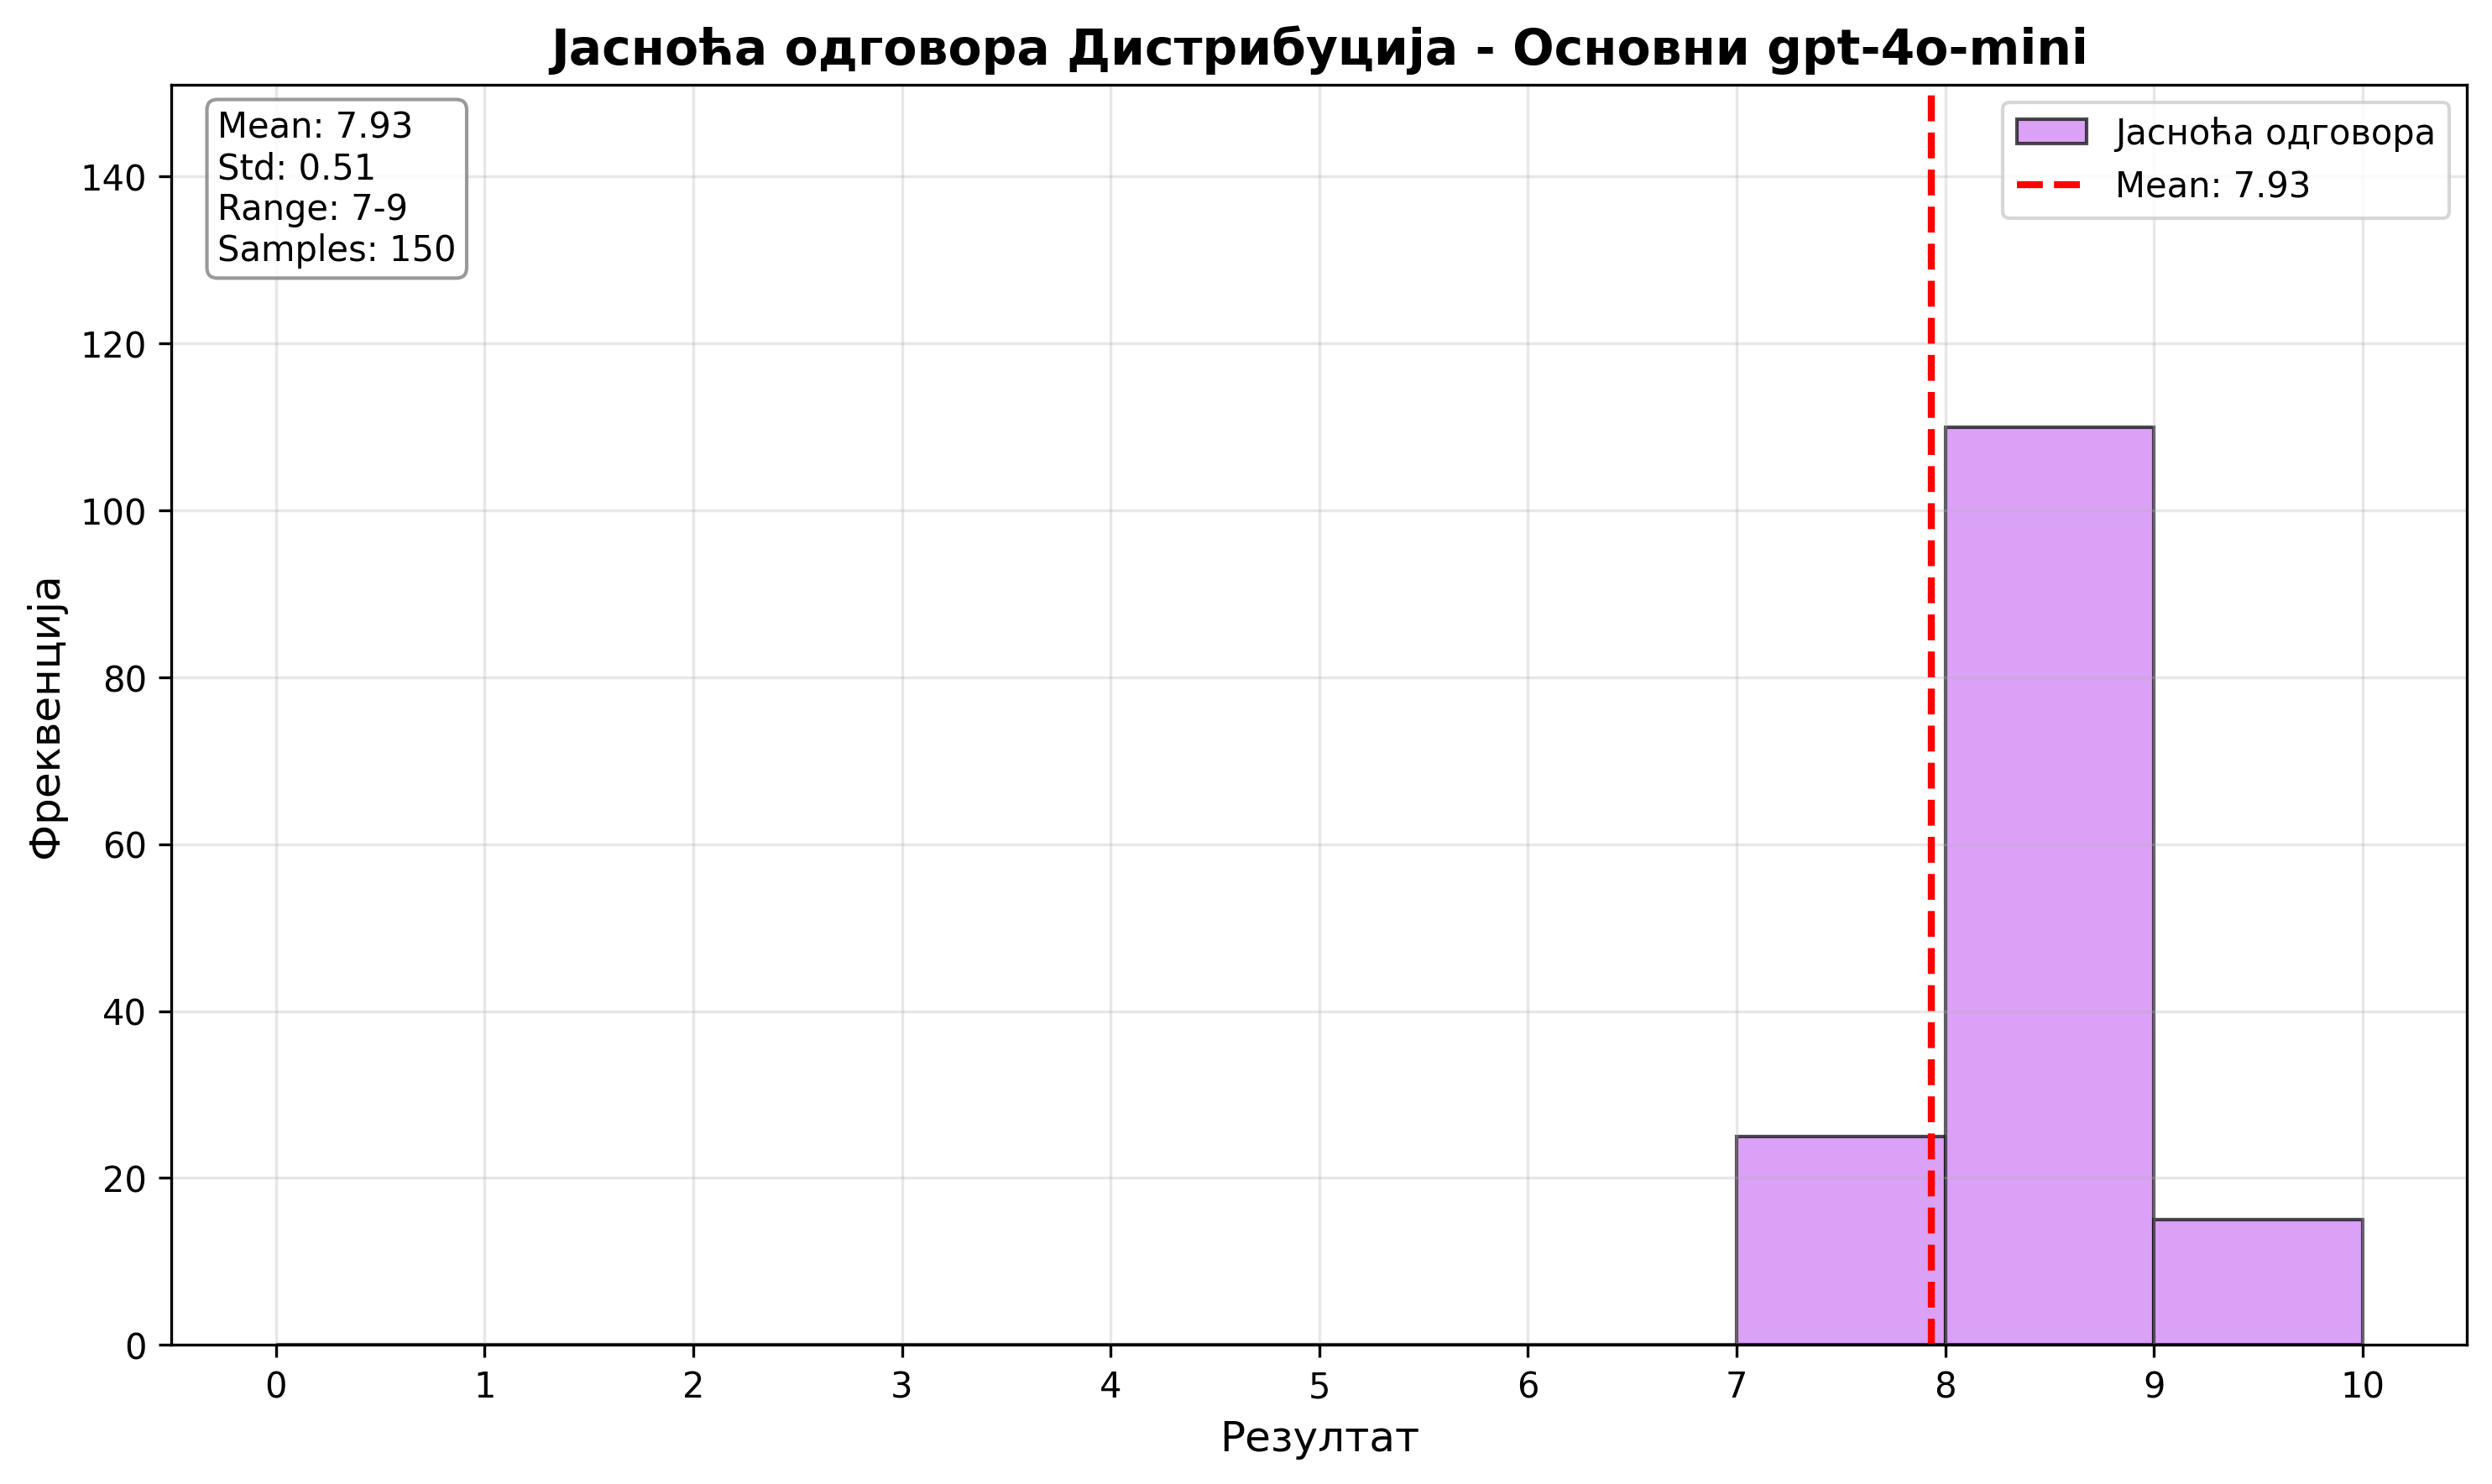
\includegraphics[width=0.8\textwidth]{images/osnovni/criteria_analysis_clarity_histogram.png}
    
    \vspace{0.5cm}
    
    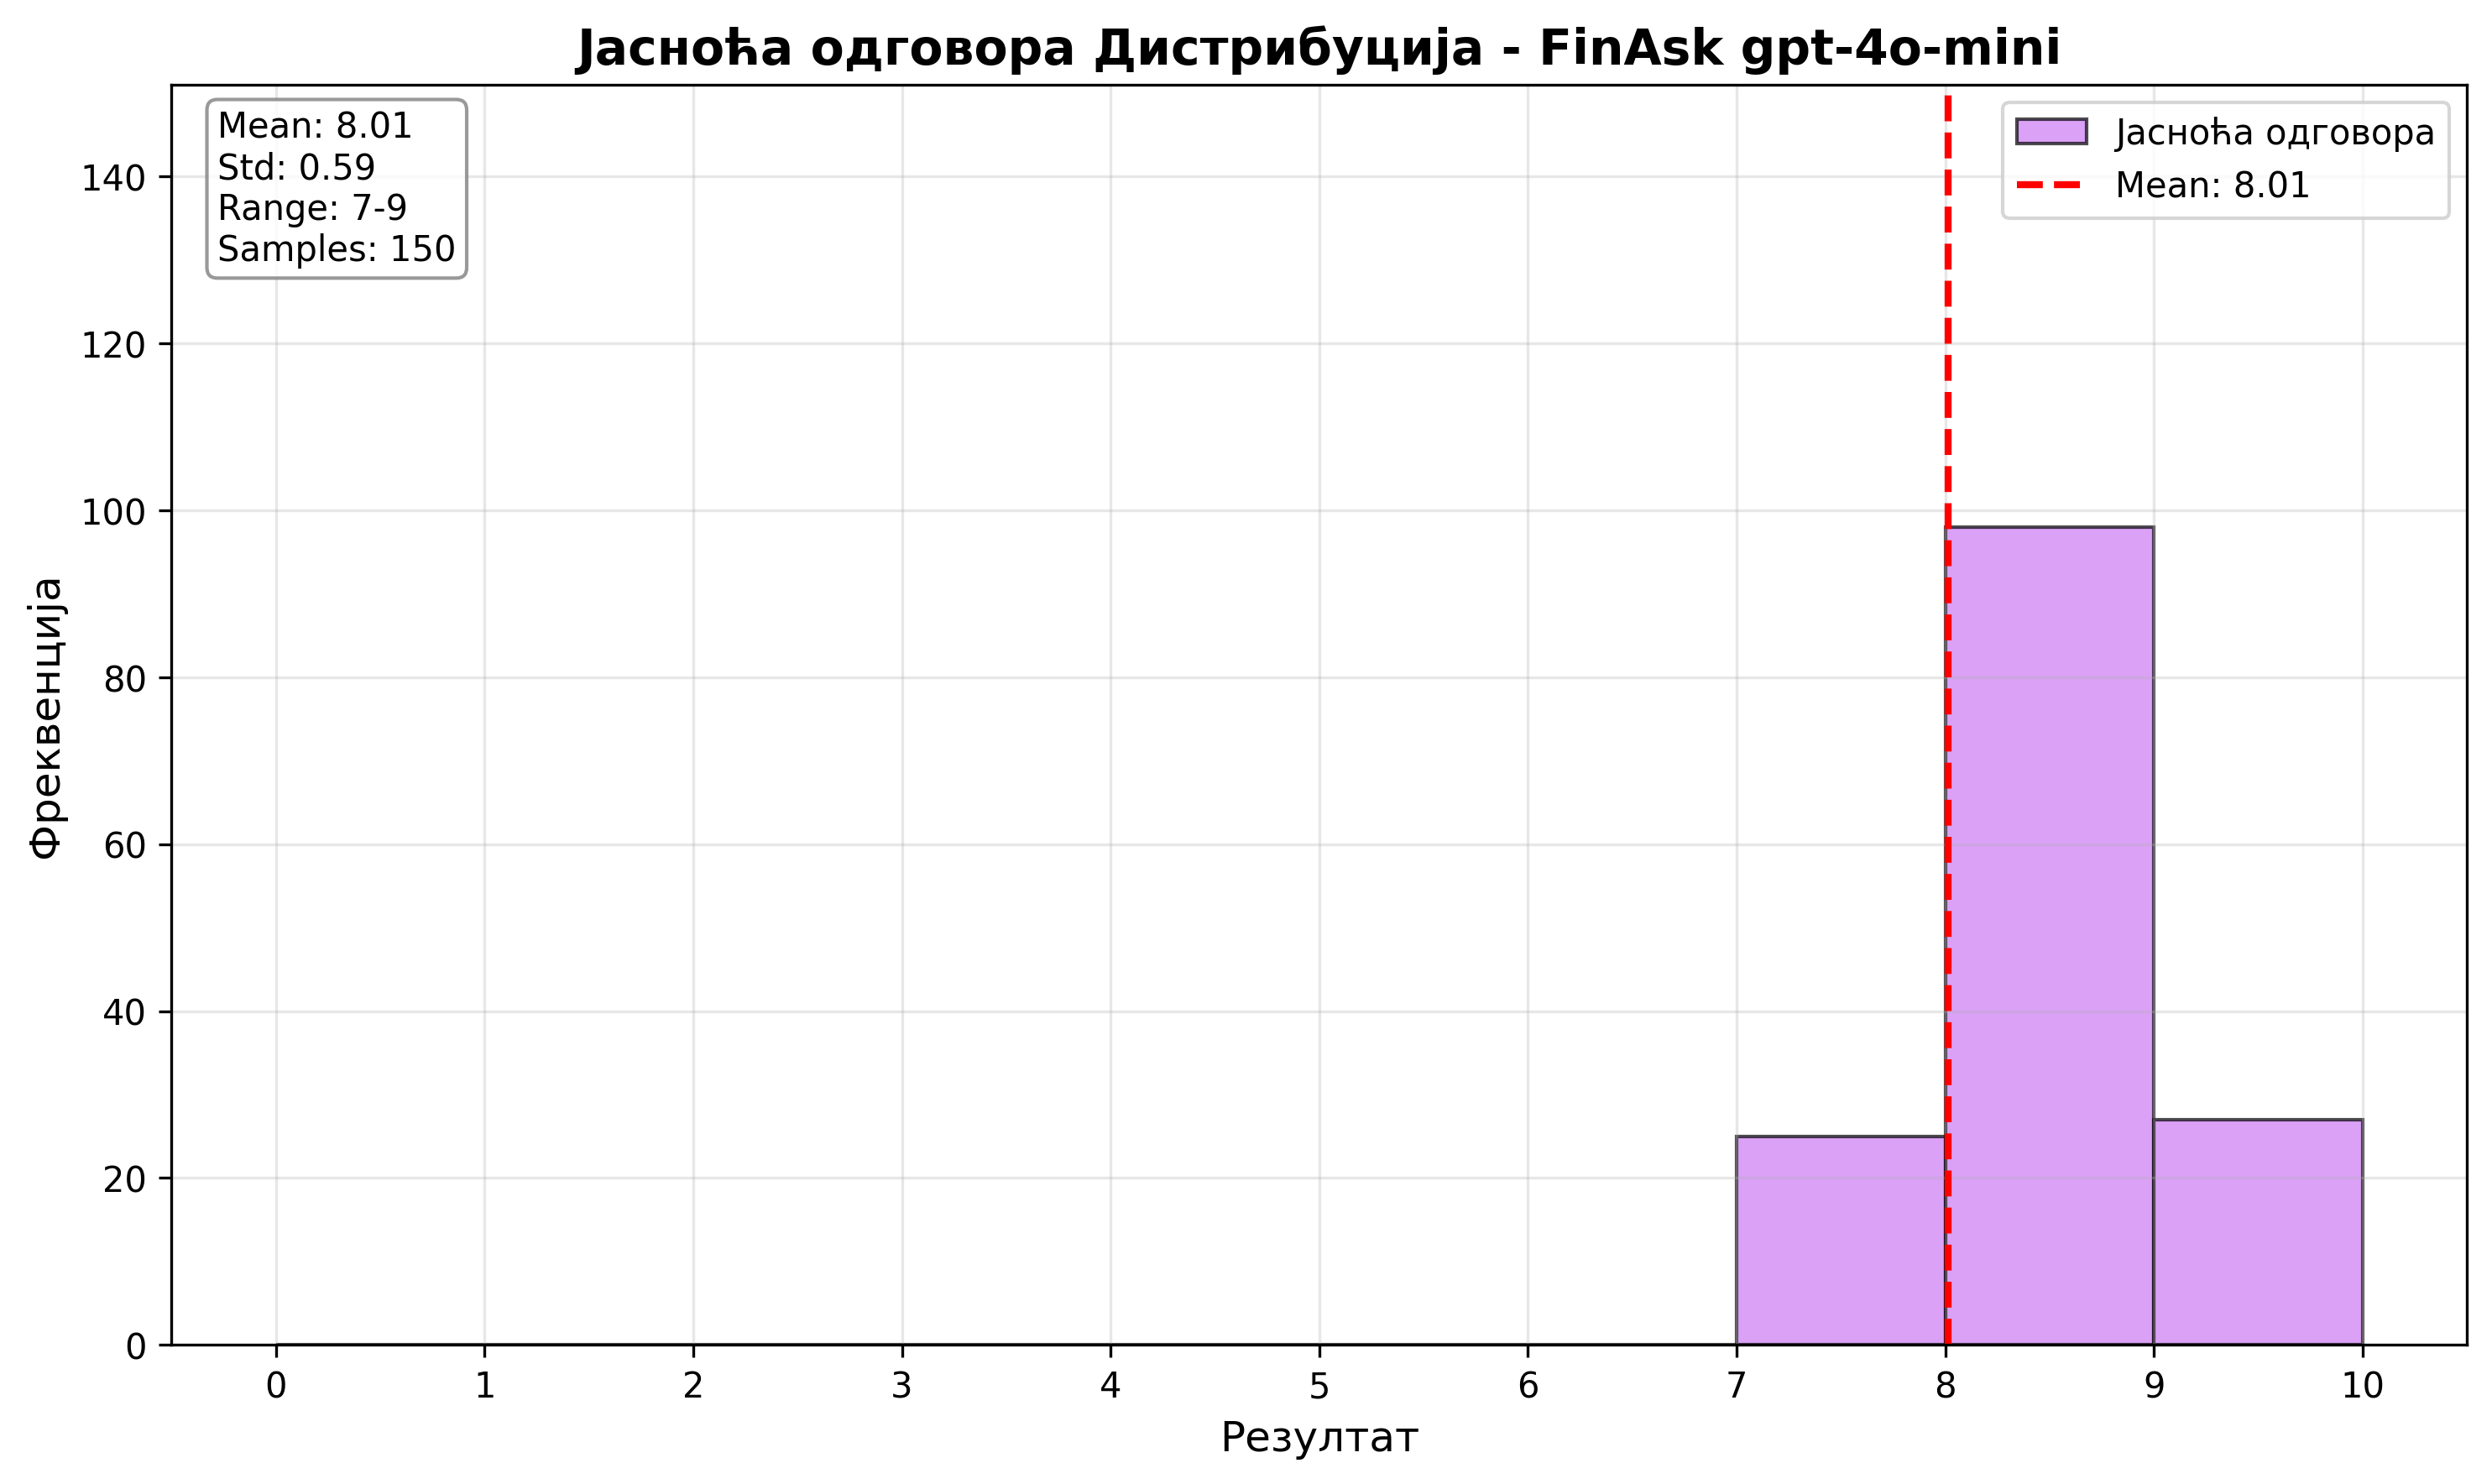
\includegraphics[width=0.8\textwidth]{images/FinAsk/criteria_analysis_clarity_histogram.png}
    \caption{Хистограм анализе критеријума јасноће - горе: основни модел, доле: FinAsk модел}
    \label{fig:comparison_clarity}
\end{figure}

\subsection{Анализа критеријума потпуности одговора}

Комплетност одговора са средњим скором од 6.41 и стандардном девијацијом од 1.03 указује на релативно конзистентну перформансу у овом домену, што сугерише да архитектура система подржава систематичан приступ структурирању одговора. У поређењу са основним моделом, FinAsk модел показује благо погоршање у просечним оценама, што указује на негативан утицај прилагођавања промпта на способност пружања обухватних анализа. Приказ поређења хистограма налази се на слици \ref{fig:comparison_completeness}.

\begin{figure}[h]
    \centering
    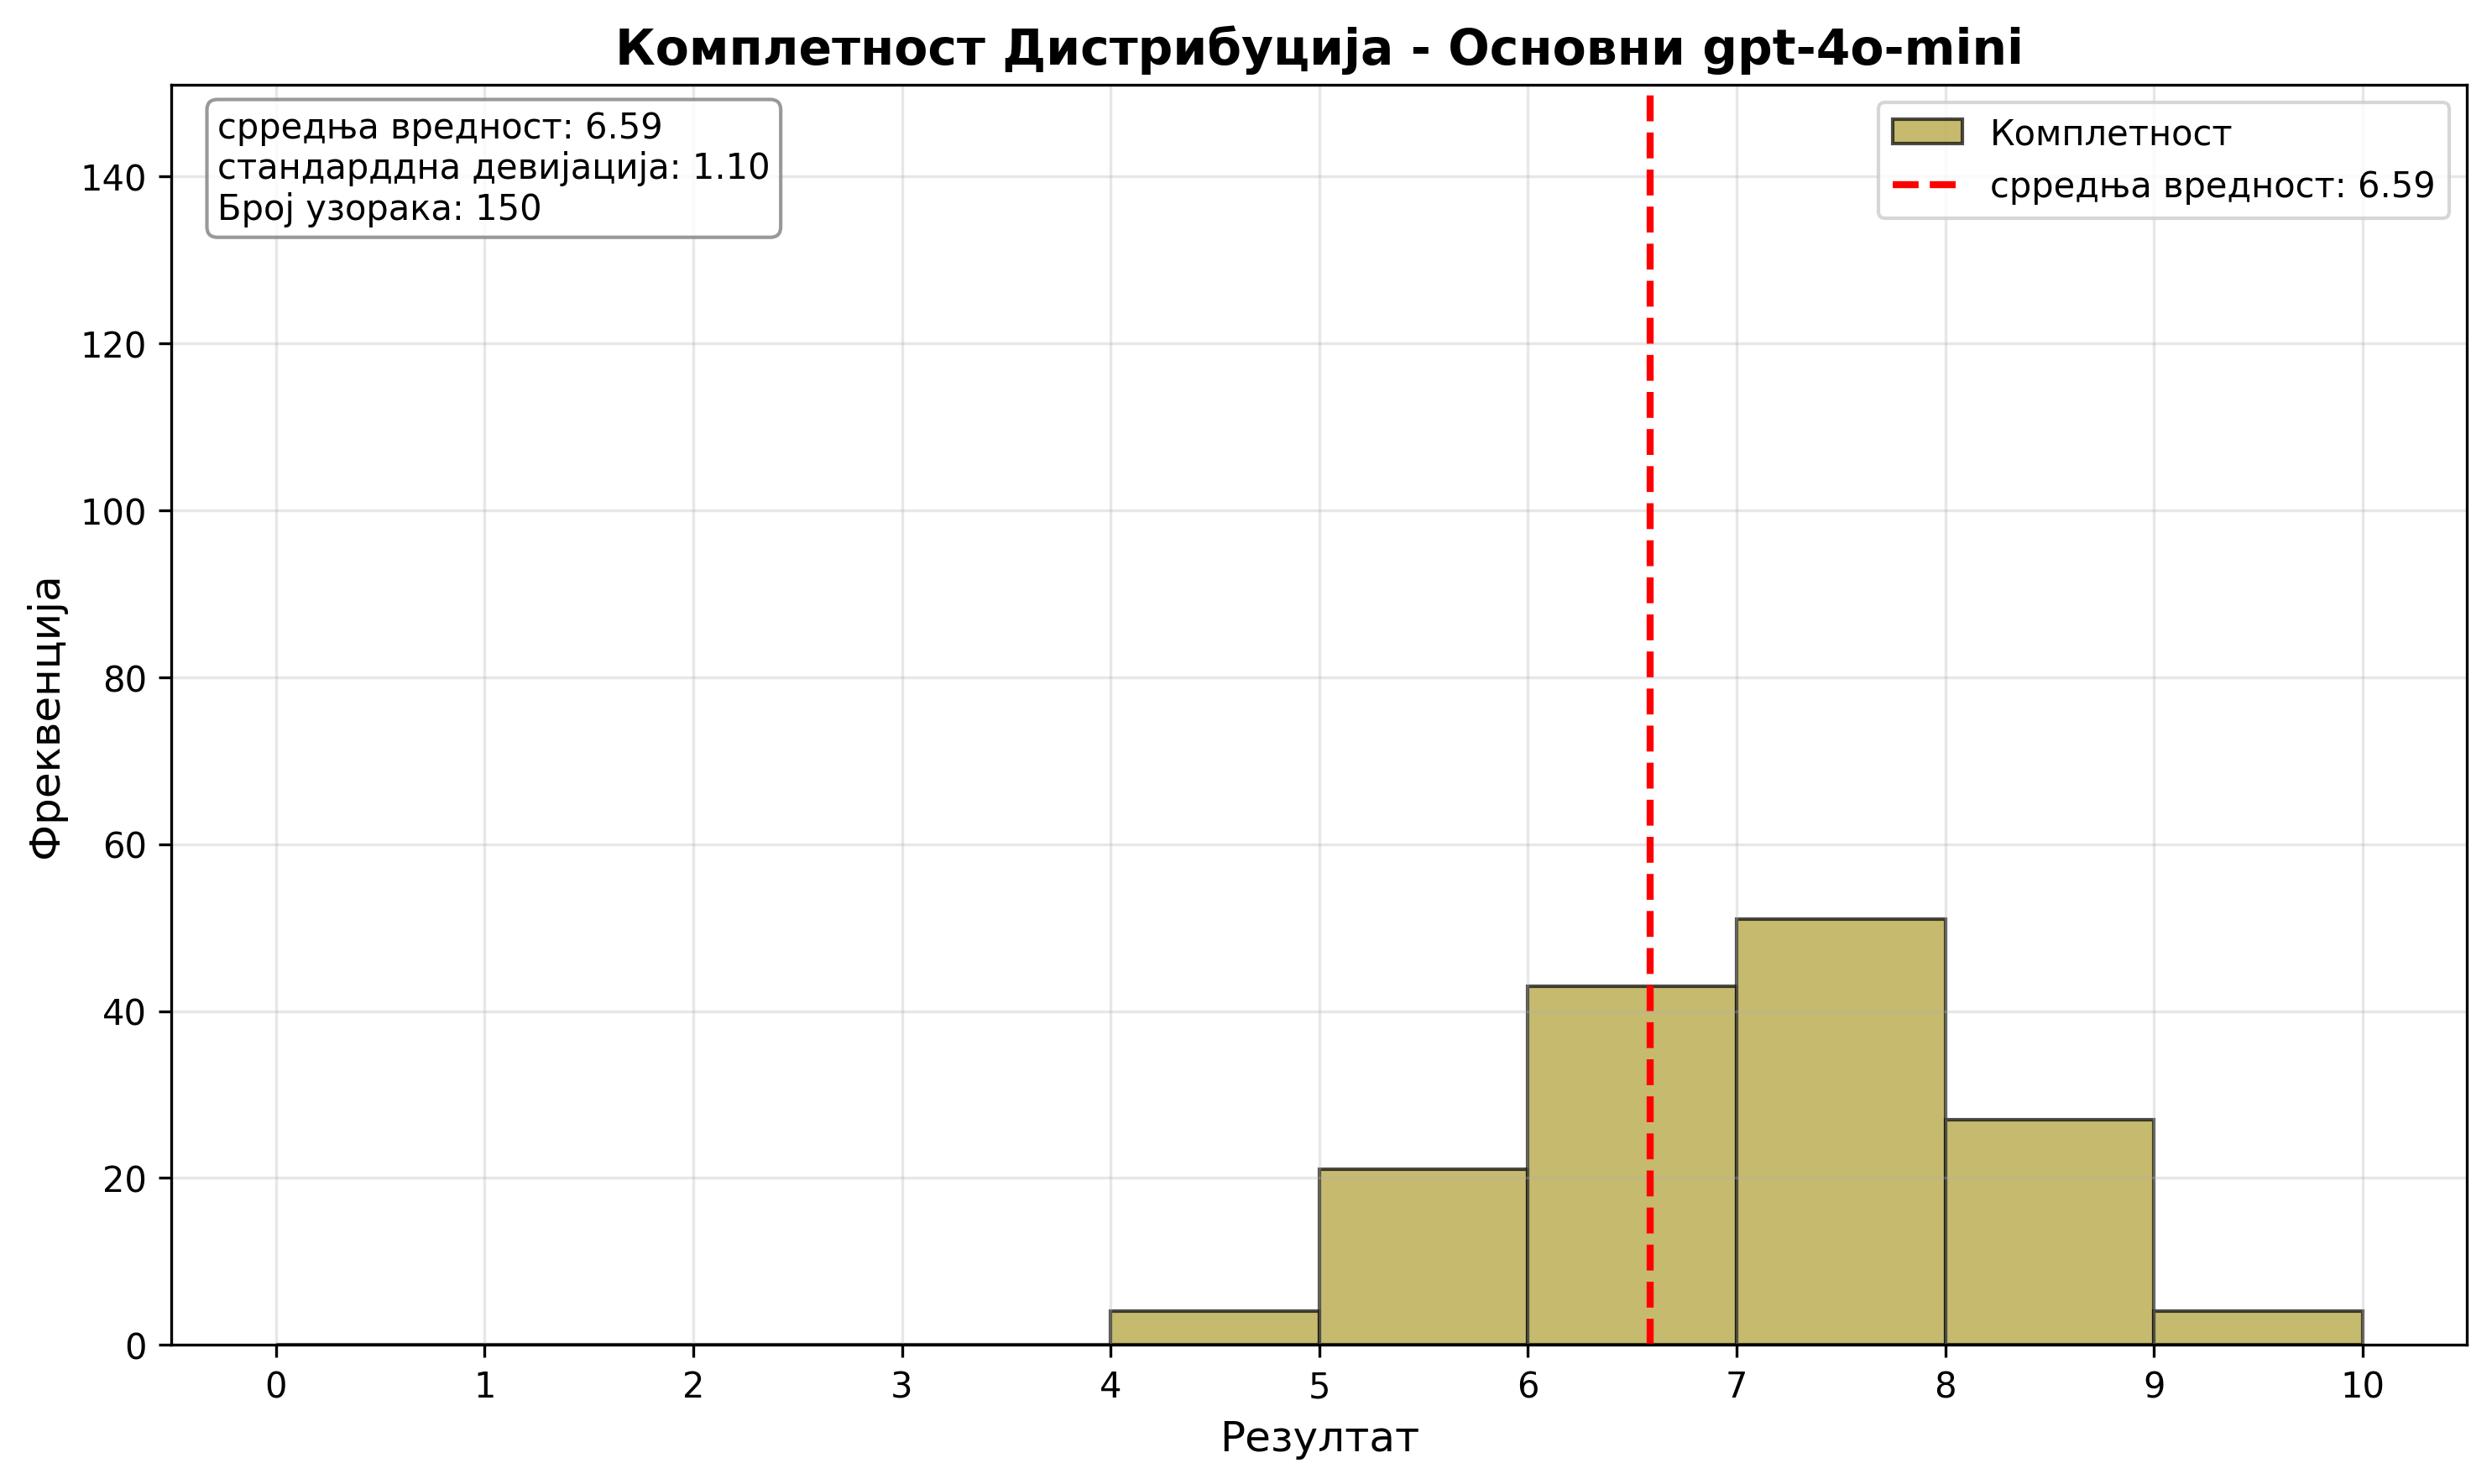
\includegraphics[width=0.8\textwidth]{images/osnovni/criteria_analysis_completeness_histogram.png}
    
    \vspace{0.5cm}
    
    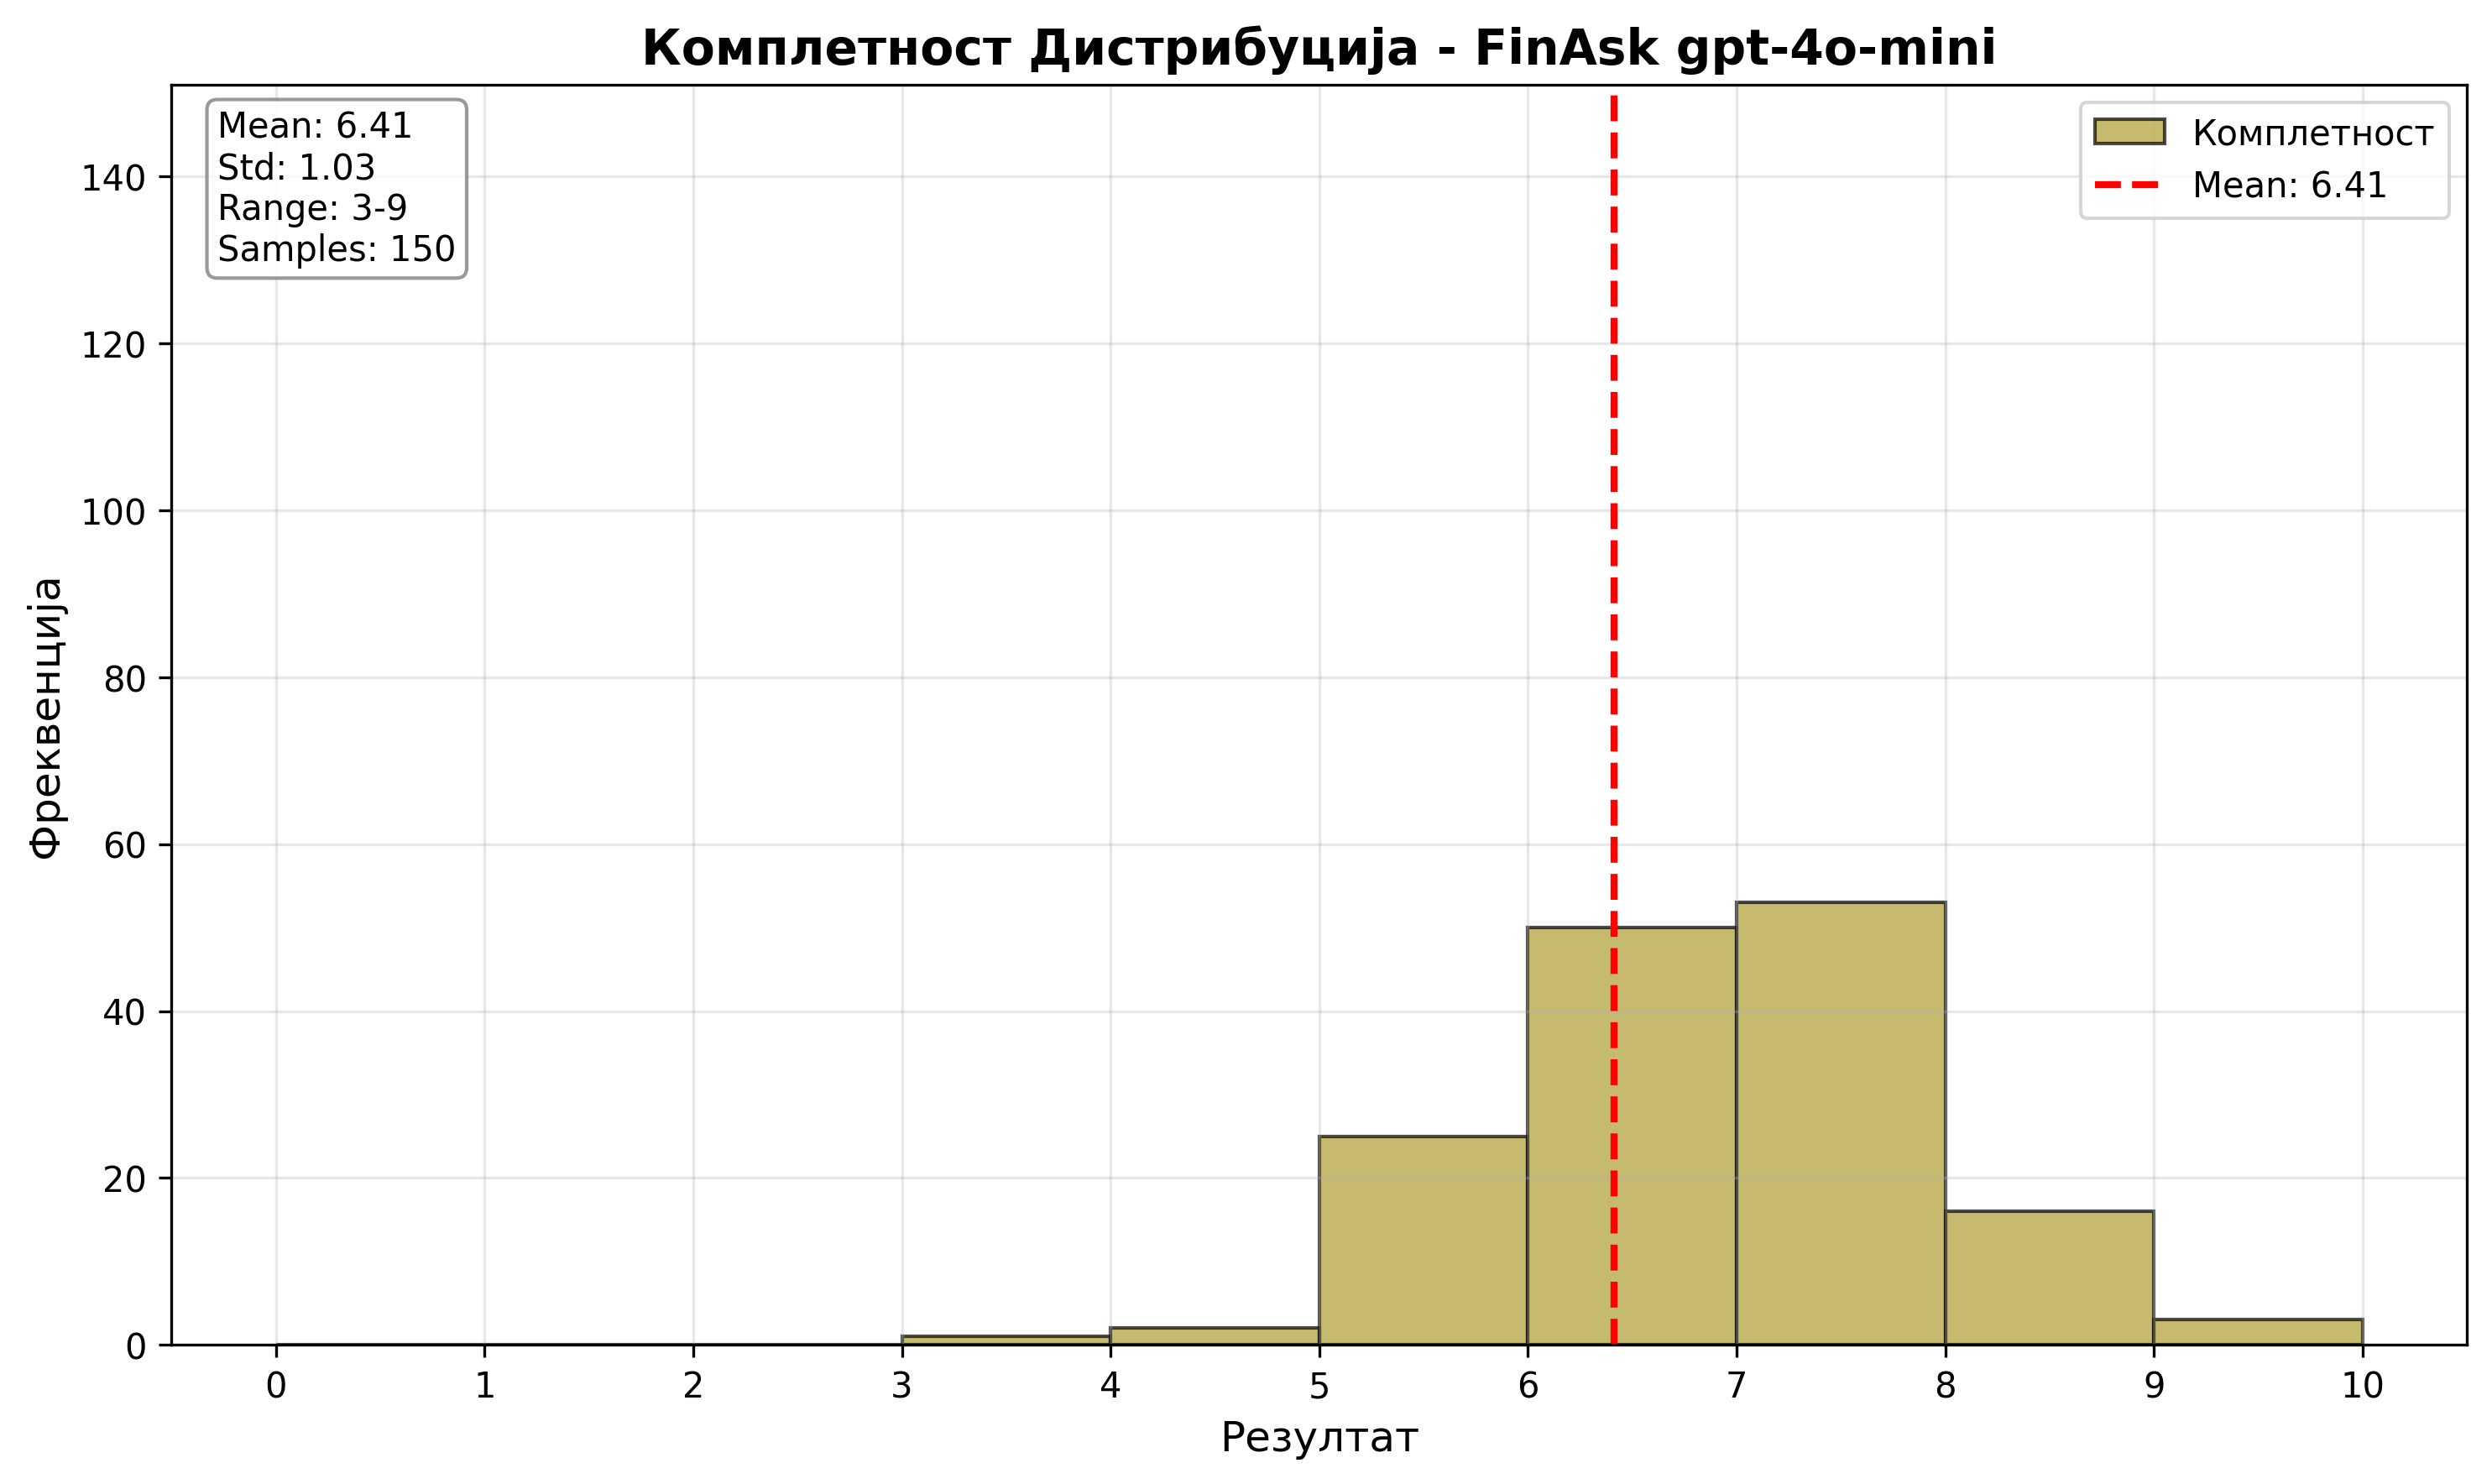
\includegraphics[width=0.8\textwidth]{images/FinAsk/criteria_analysis_completeness_histogram.png}
    \caption{Хистограм анализе критеријума потпуности - горе: основни модел, доле: FinAsk модел}
    \label{fig:comparison_completeness}
\end{figure}

\subsection{Анализа критеријума тачности}

Фактуална исправност са просечним скором од 5.09 и стандардном девијацијом од 1.26 представља умерен ниво тачности који сугерише да систем успева да идентификује и репродукује релевантне финансијске информације у приближно половини случајева. Ова метрика је кључна за практичну примену система јер директно утиче на поверење корисника и употребљивост у реалним сценаријима финансијског саветовања. Релативно висока варијабилност указује на недоследност у приступу обради различитих типова упита, што може бити последица ограничења у основном језичком моделу или недовољне оптимизације промпт инжењеринга. У односу на основни модел приметно је велико побољшање што говори да основни модел нема информације које су потребне за тачан одговор, а FinAsk модел их успешно проналази. Додатно, ово показује способност агент асудије да распознаје и награди тачне одговоре. Приказ поређења хистограма налази се на слици \ref{fig:comparison_factual}.

\begin{figure}[h]
    \centering
    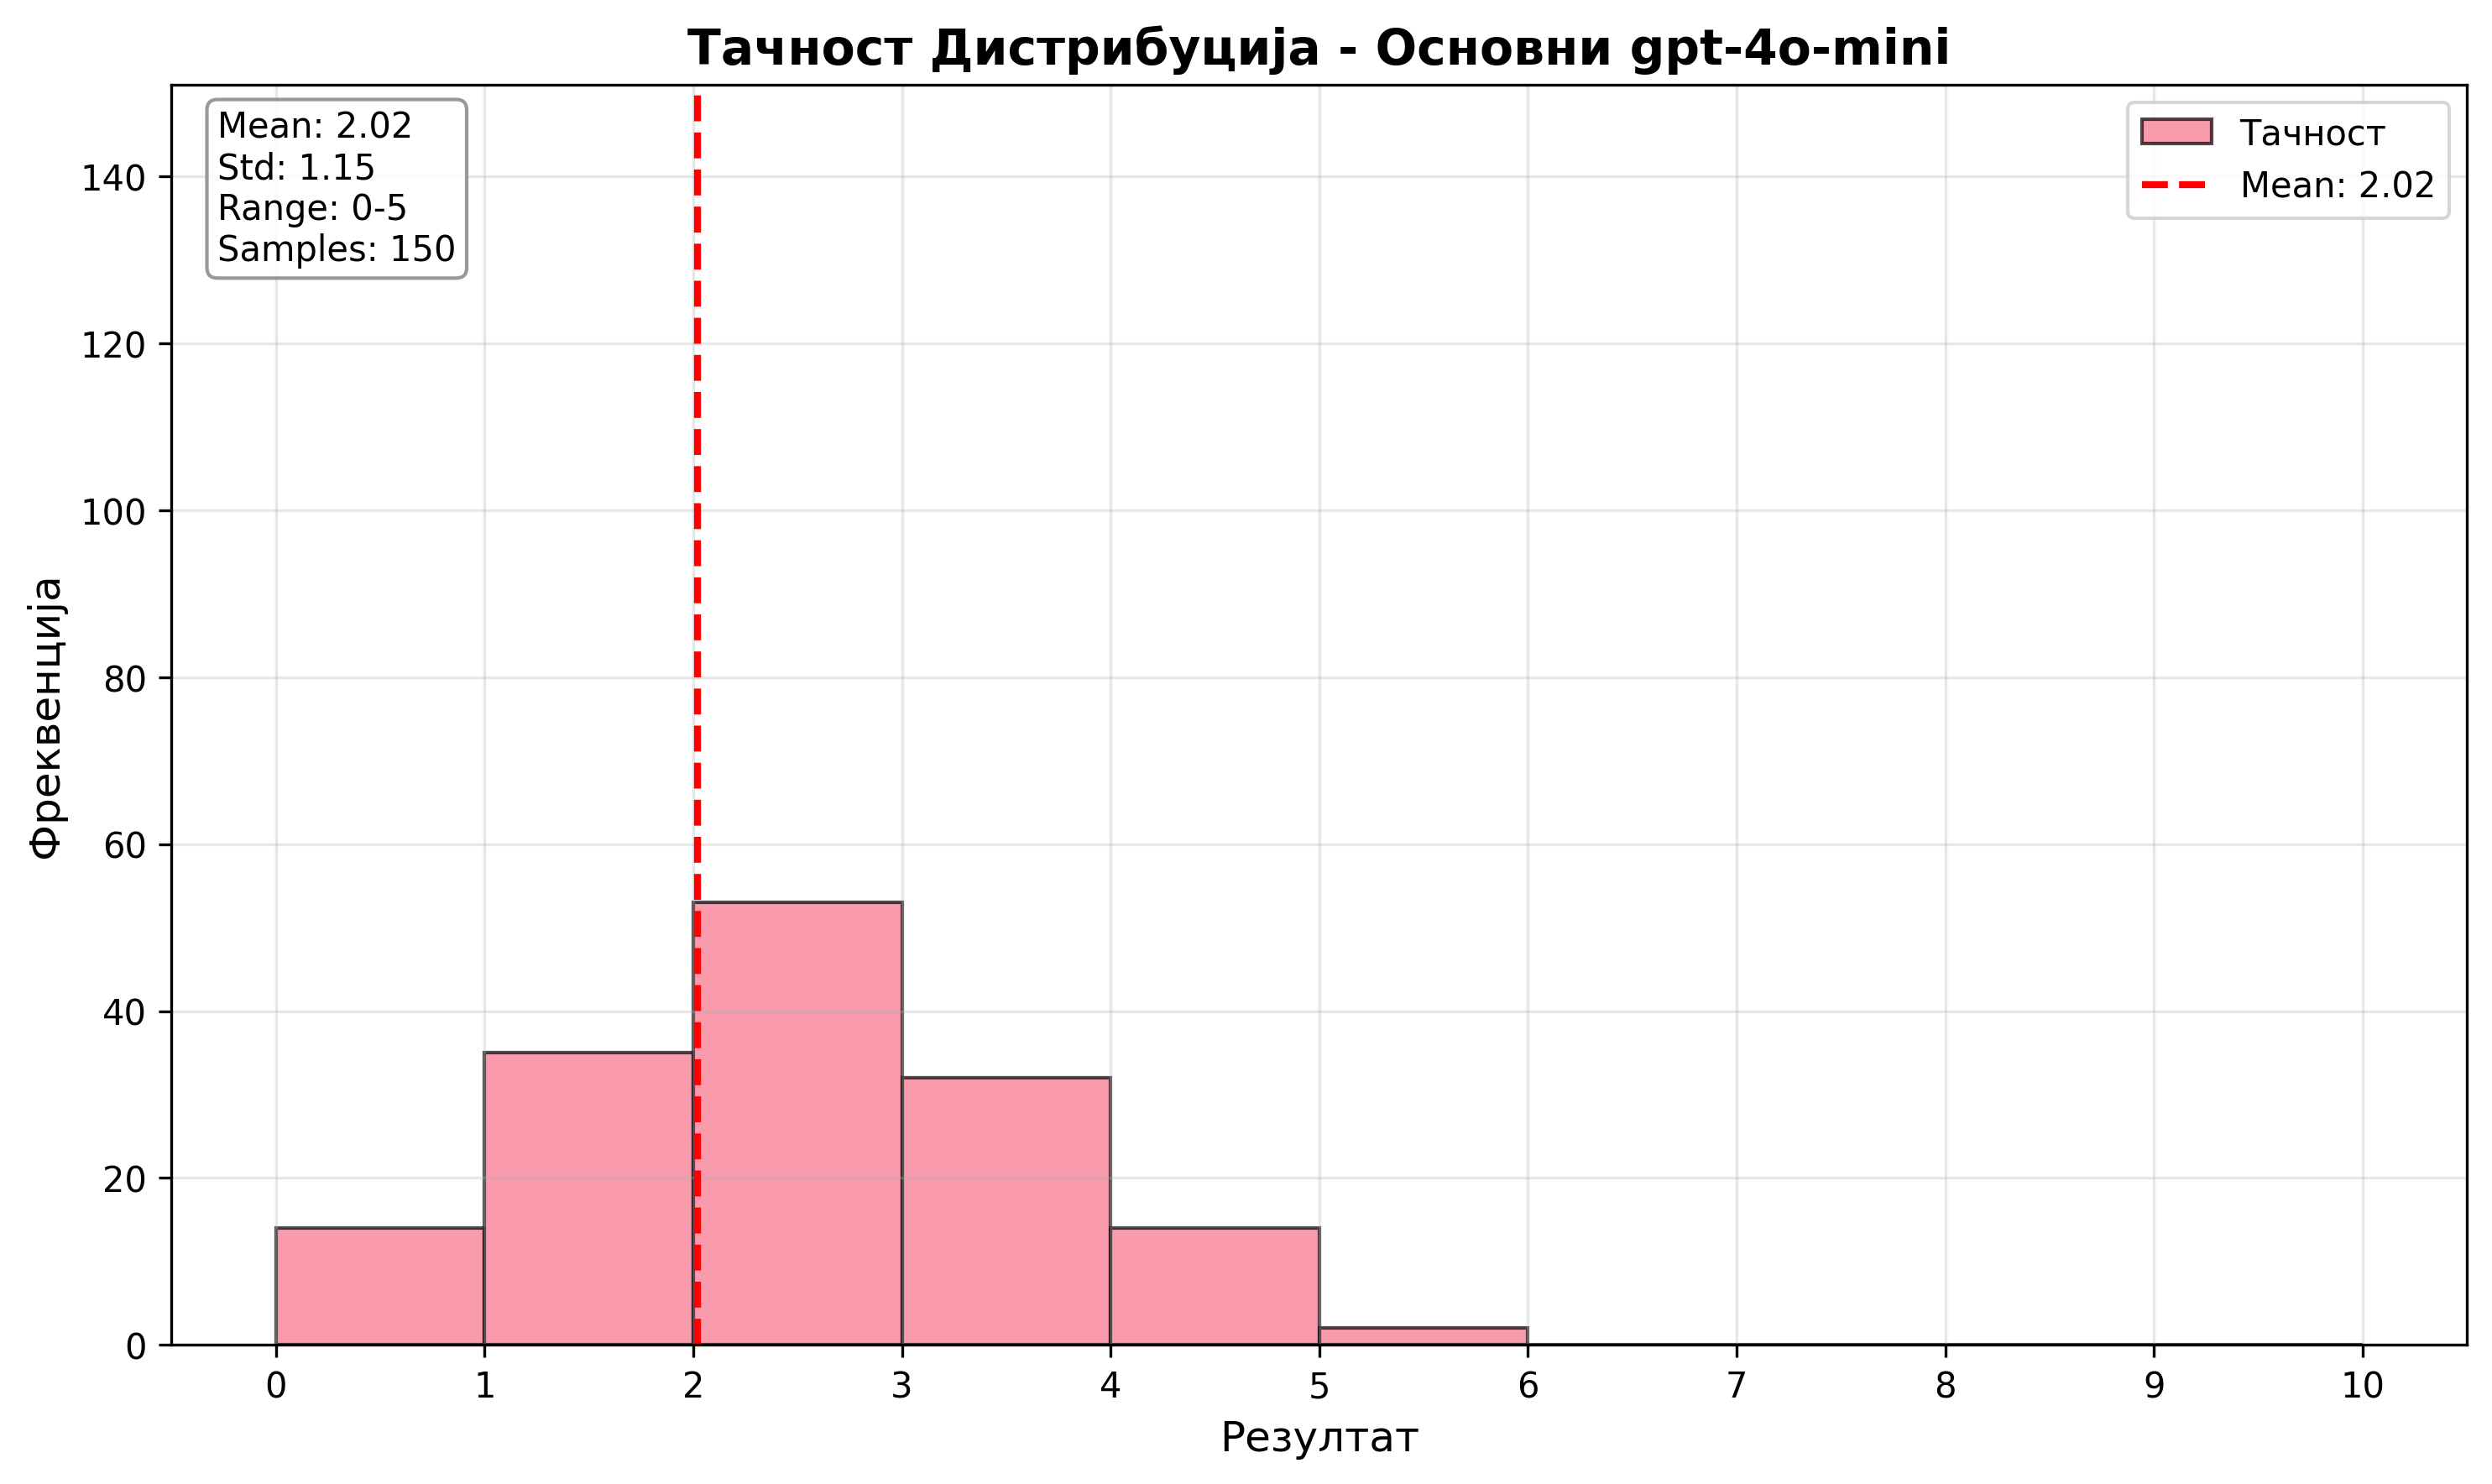
\includegraphics[width=0.8\textwidth]{images/osnovni/criteria_analysis_factual_correctness_histogram.png}
    
    \vspace{0.5cm}
    
    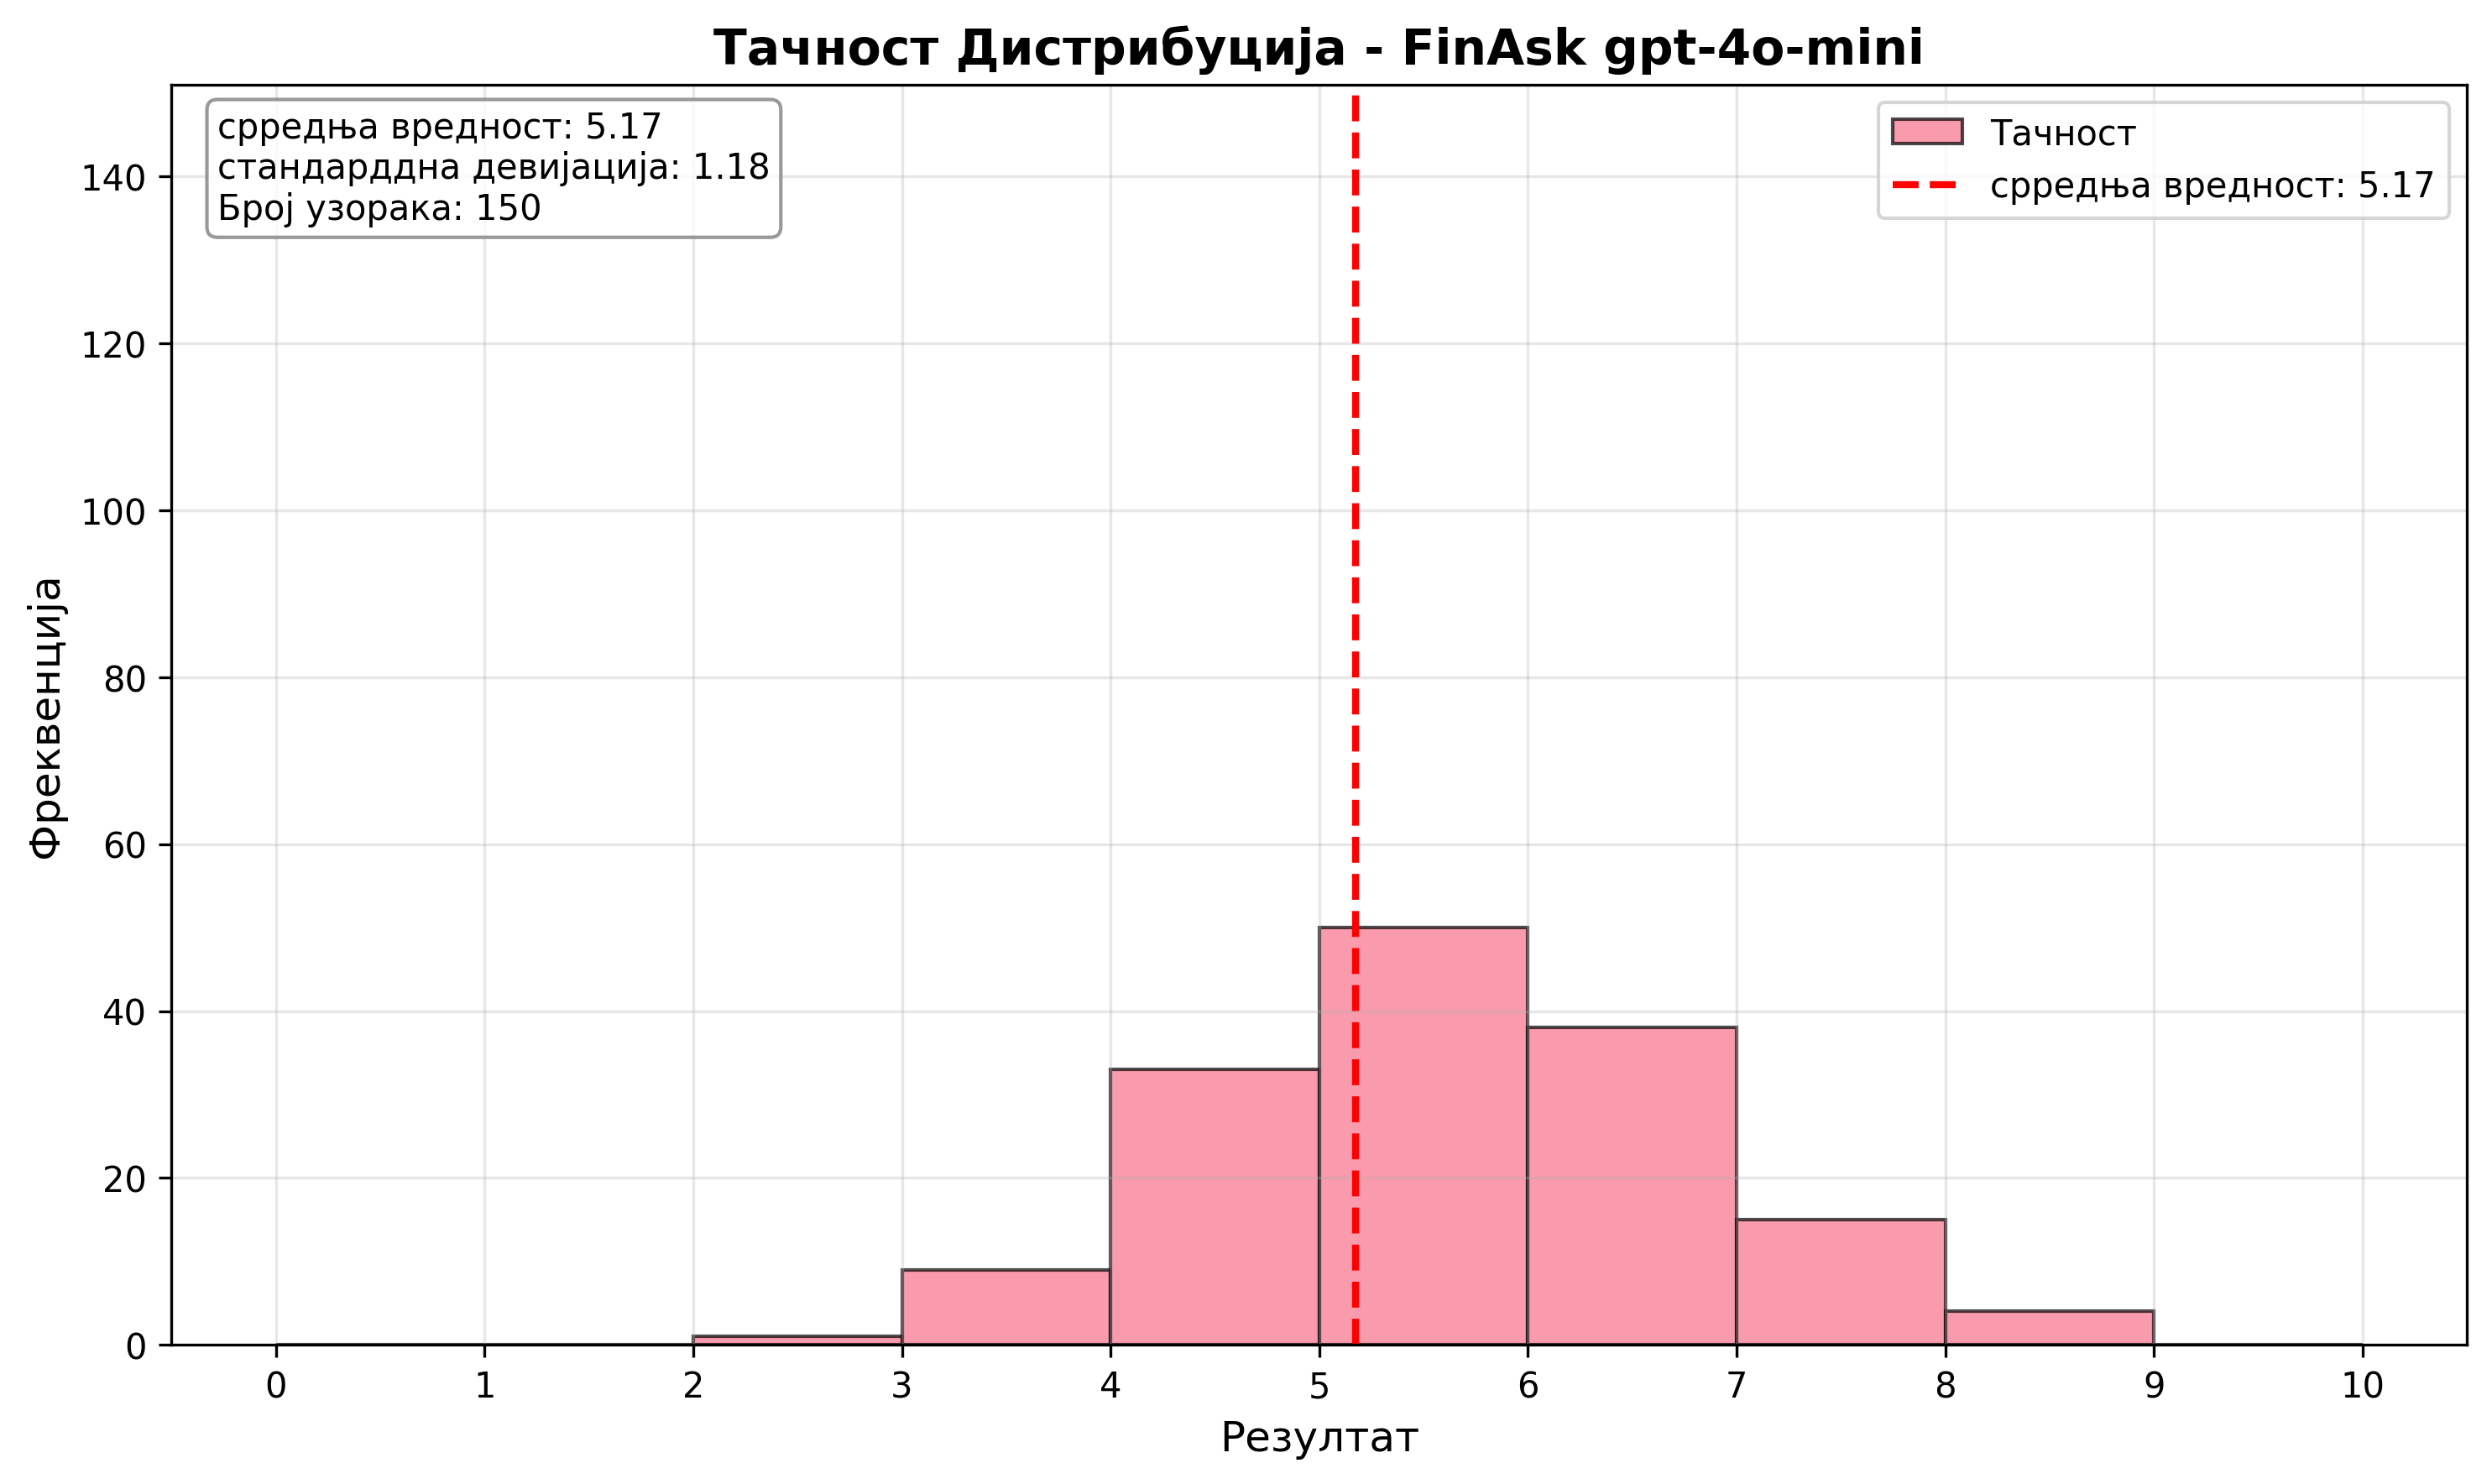
\includegraphics[width=0.8\textwidth]{images/FinAsk/criteria_analysis_factual_correctness_histogram.png}
    \caption{Хистограм анализе критеријума фактичке тачности - горе: основни модел, доле: FinAsk модел}
    \label{fig:comparison_factual}
\end{figure}

\subsection{Анализа критеријума финансијског резоновања}

К Финансијско резоновање са скором од 7.97 представља један од најснажнијих аспеката система, указујући на способност извођења логичких закључака и примене финансијских принципа у анализи. Ова висока перформанса је посебно значајна јер одражава дубину разумевања финансијских концепата и способност њихове примене у различитим контекстовима. Међутим, разлика у скору између основног модела и FinAsk модела је минимална, што указује да прилагођавање промпта није донело значајно побољшање у овој области. Поставља се питање да ли прилагођавање промпта може утицати на дубину финансијског резоновања или су ове способности уграђене у основни језички модел. Приказ поређења хистограма налази се на слици \ref{fig:comparison_financial}.

\begin{figure}[h]
    \centering
    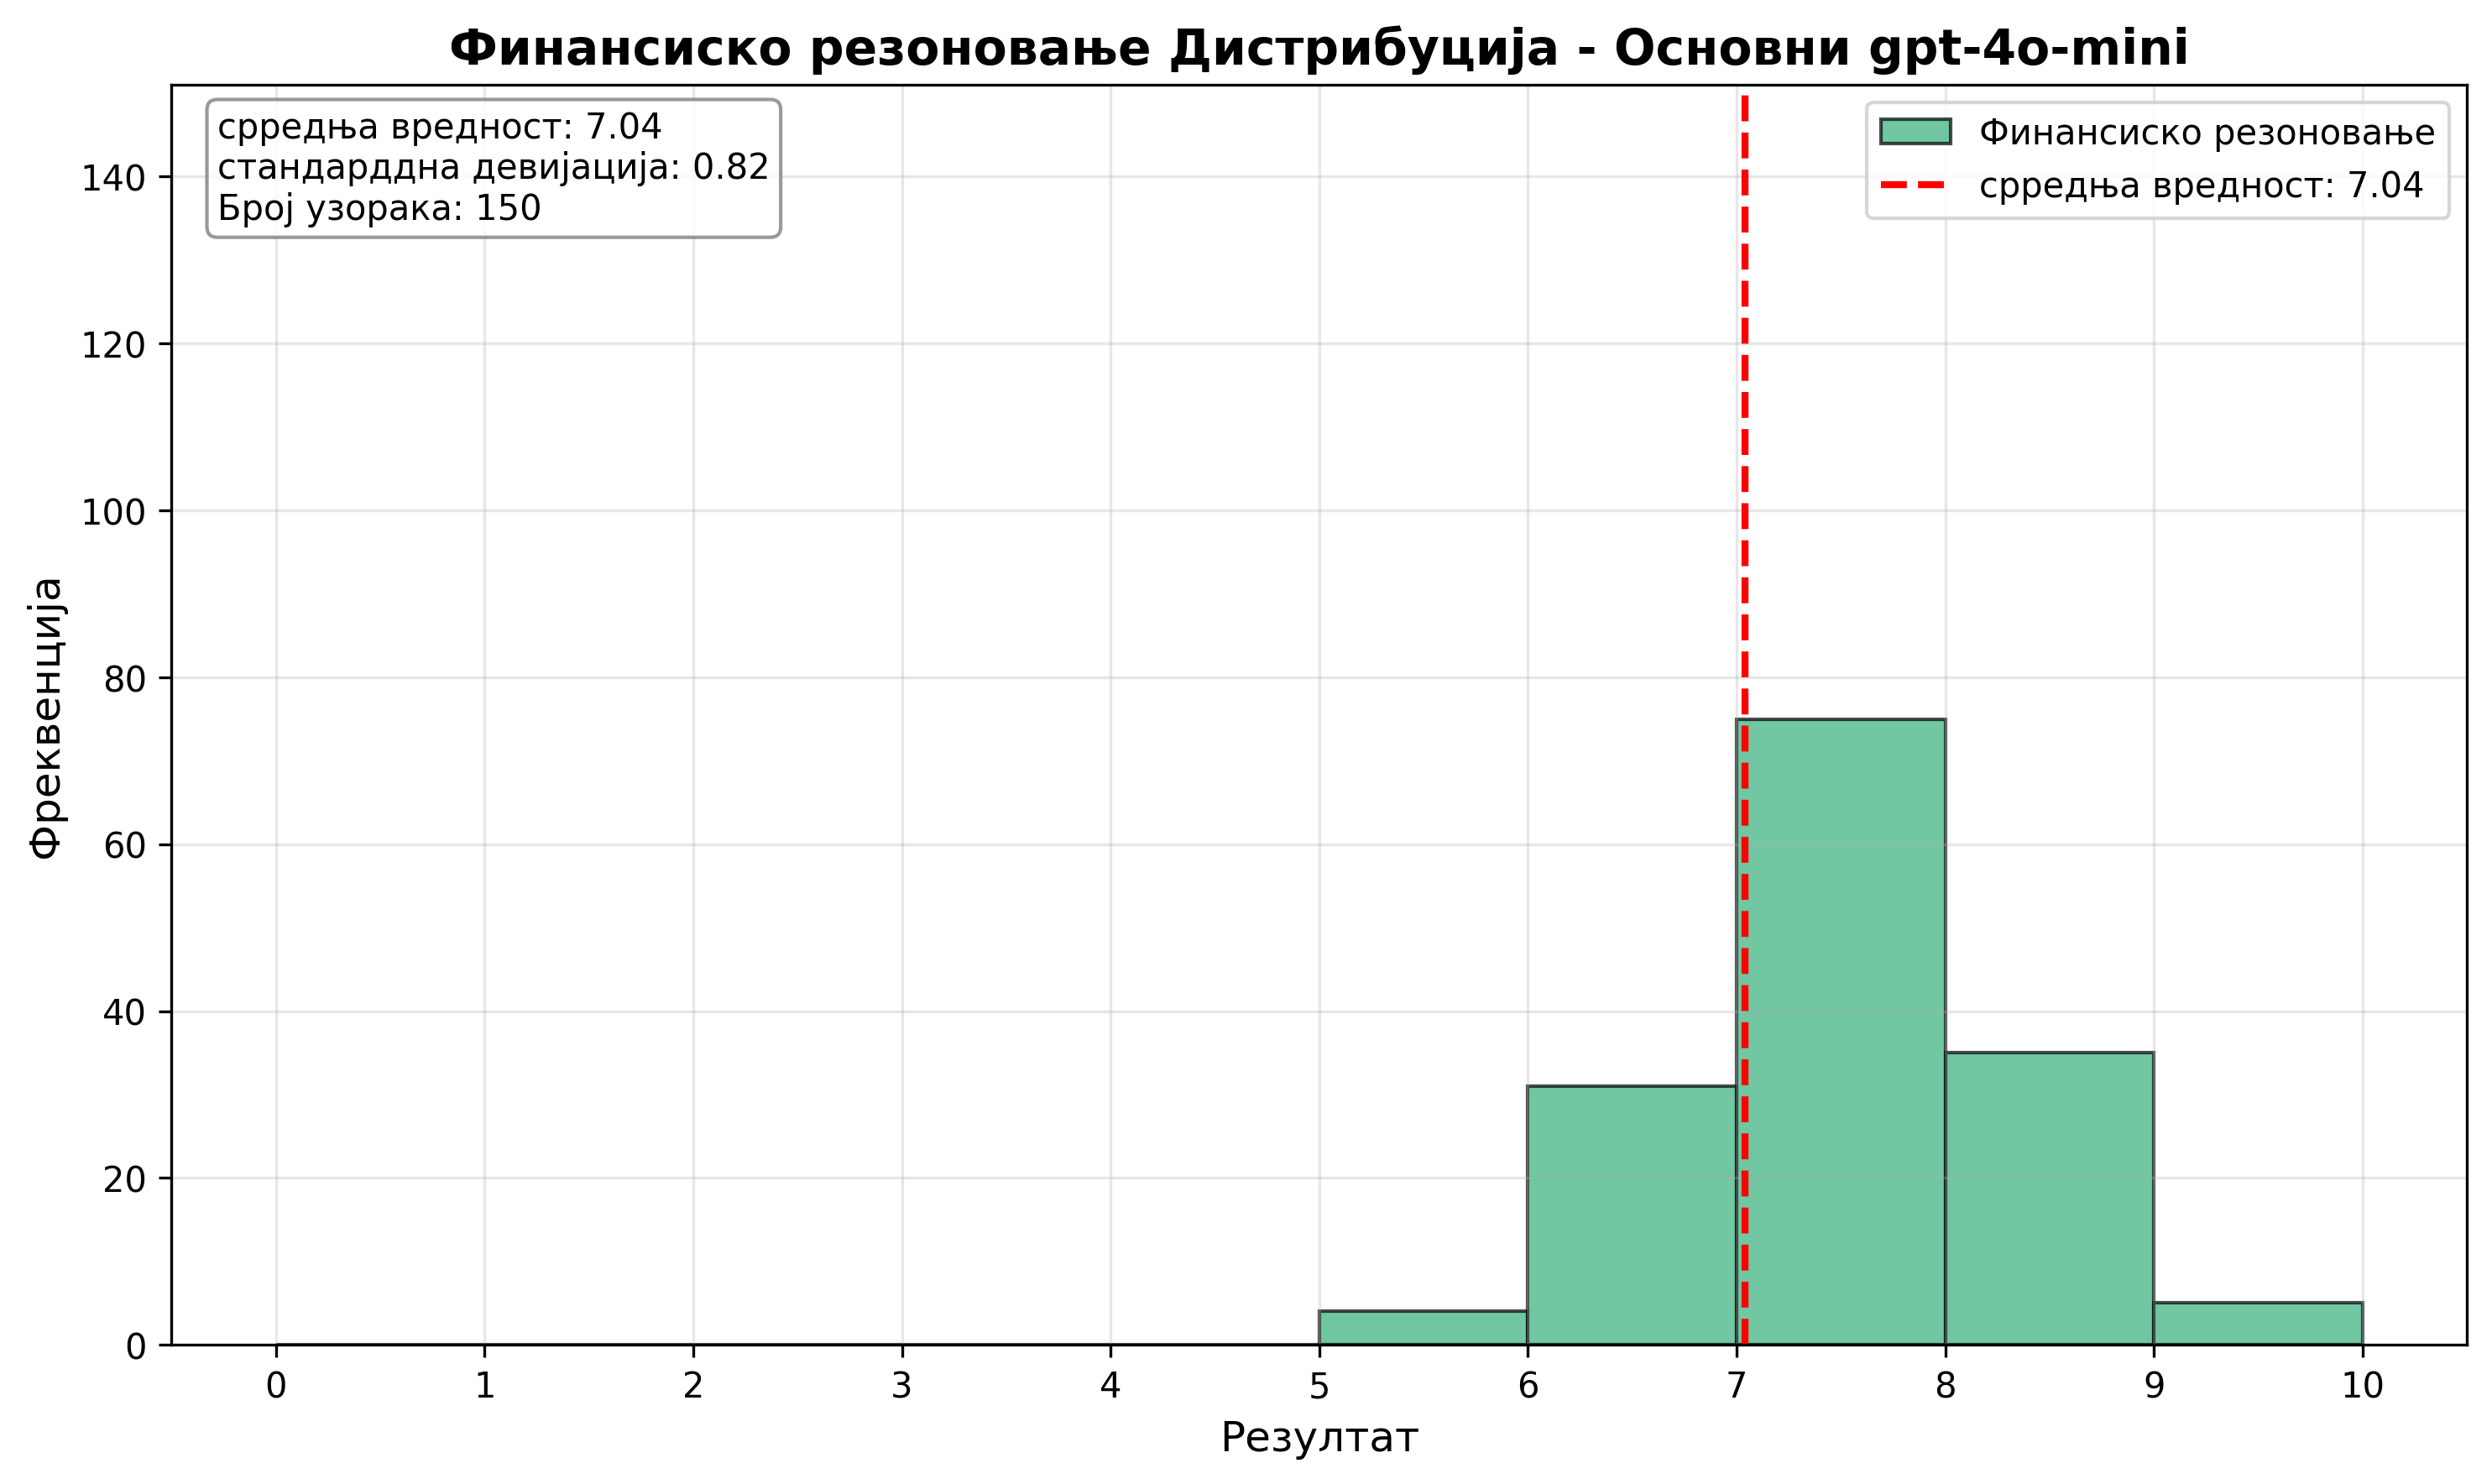
\includegraphics[width=0.8\textwidth]{images/osnovni/criteria_analysis_financial_reasoning_histogram.png}
    
    \vspace{0.5cm}
    
    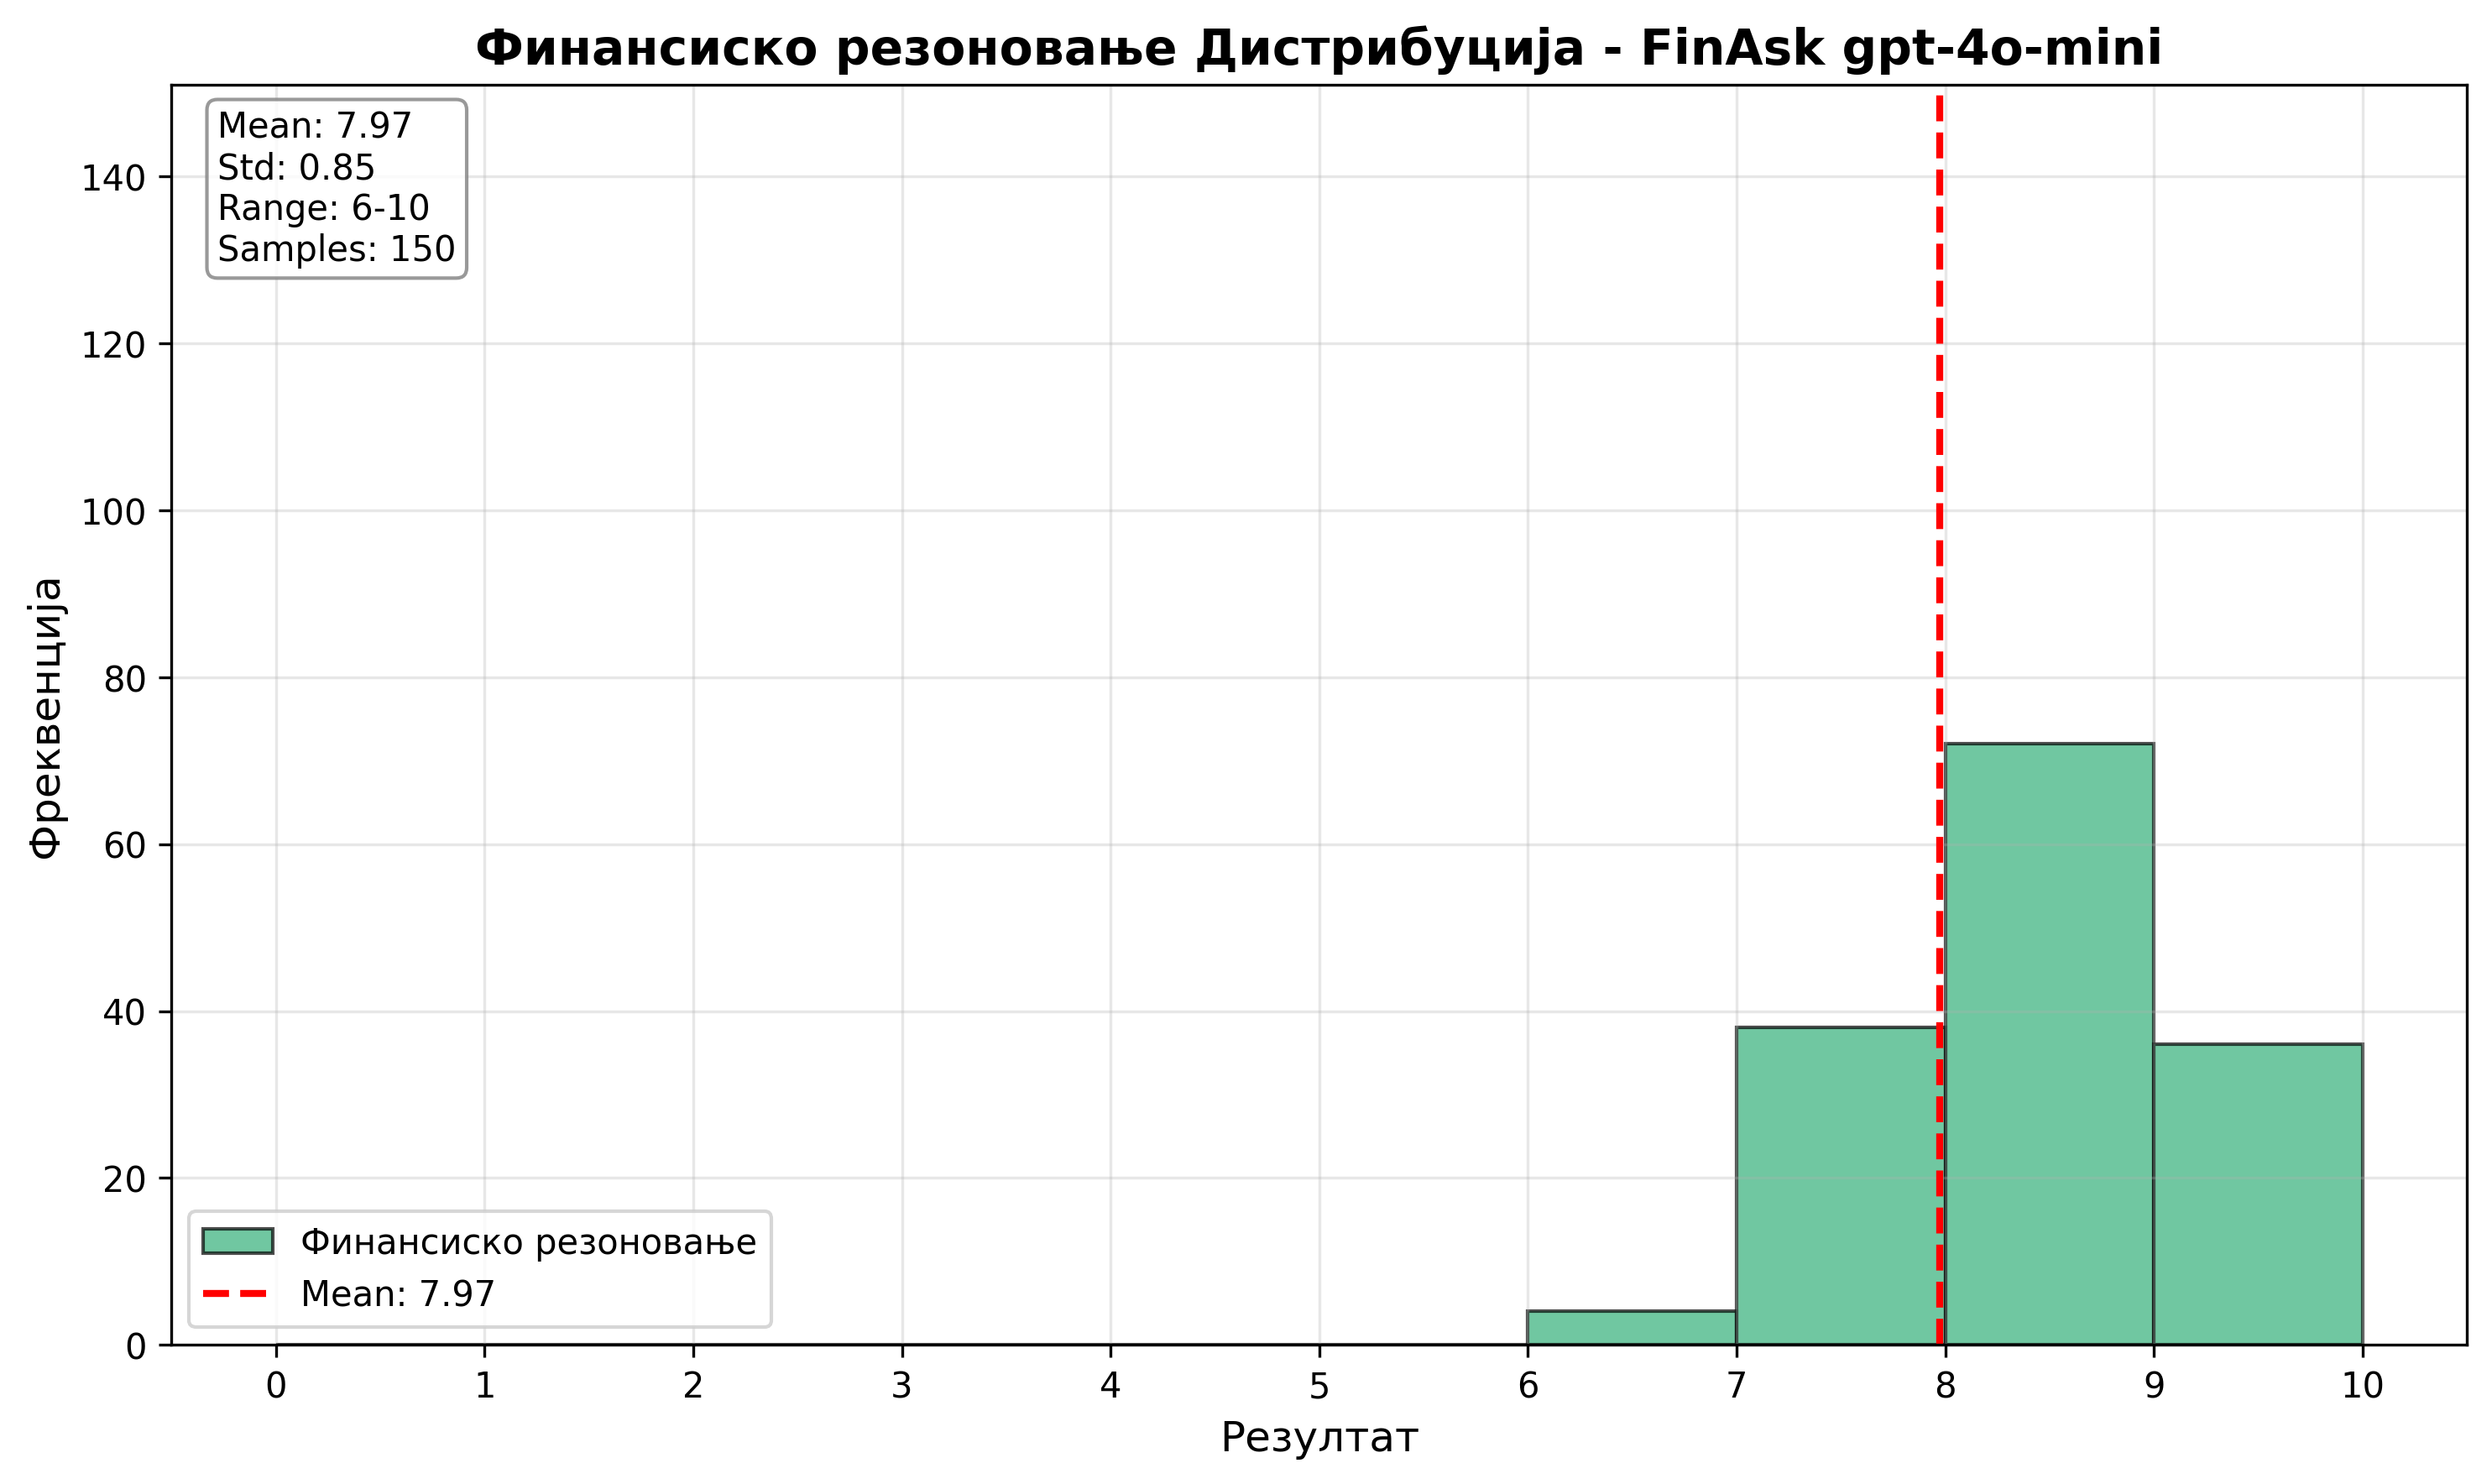
\includegraphics[width=0.8\textwidth]{images/FinAsk/criteria_analysis_financial_reasoning_histogram.png}
    \caption{Хистограм анализе критеријума финансијског резоновања - горе: основни модел, доле: FinAsk модел}
    \label{fig:comparison_financial}
\end{figure}

\begin{figure}[h]
    \centering
    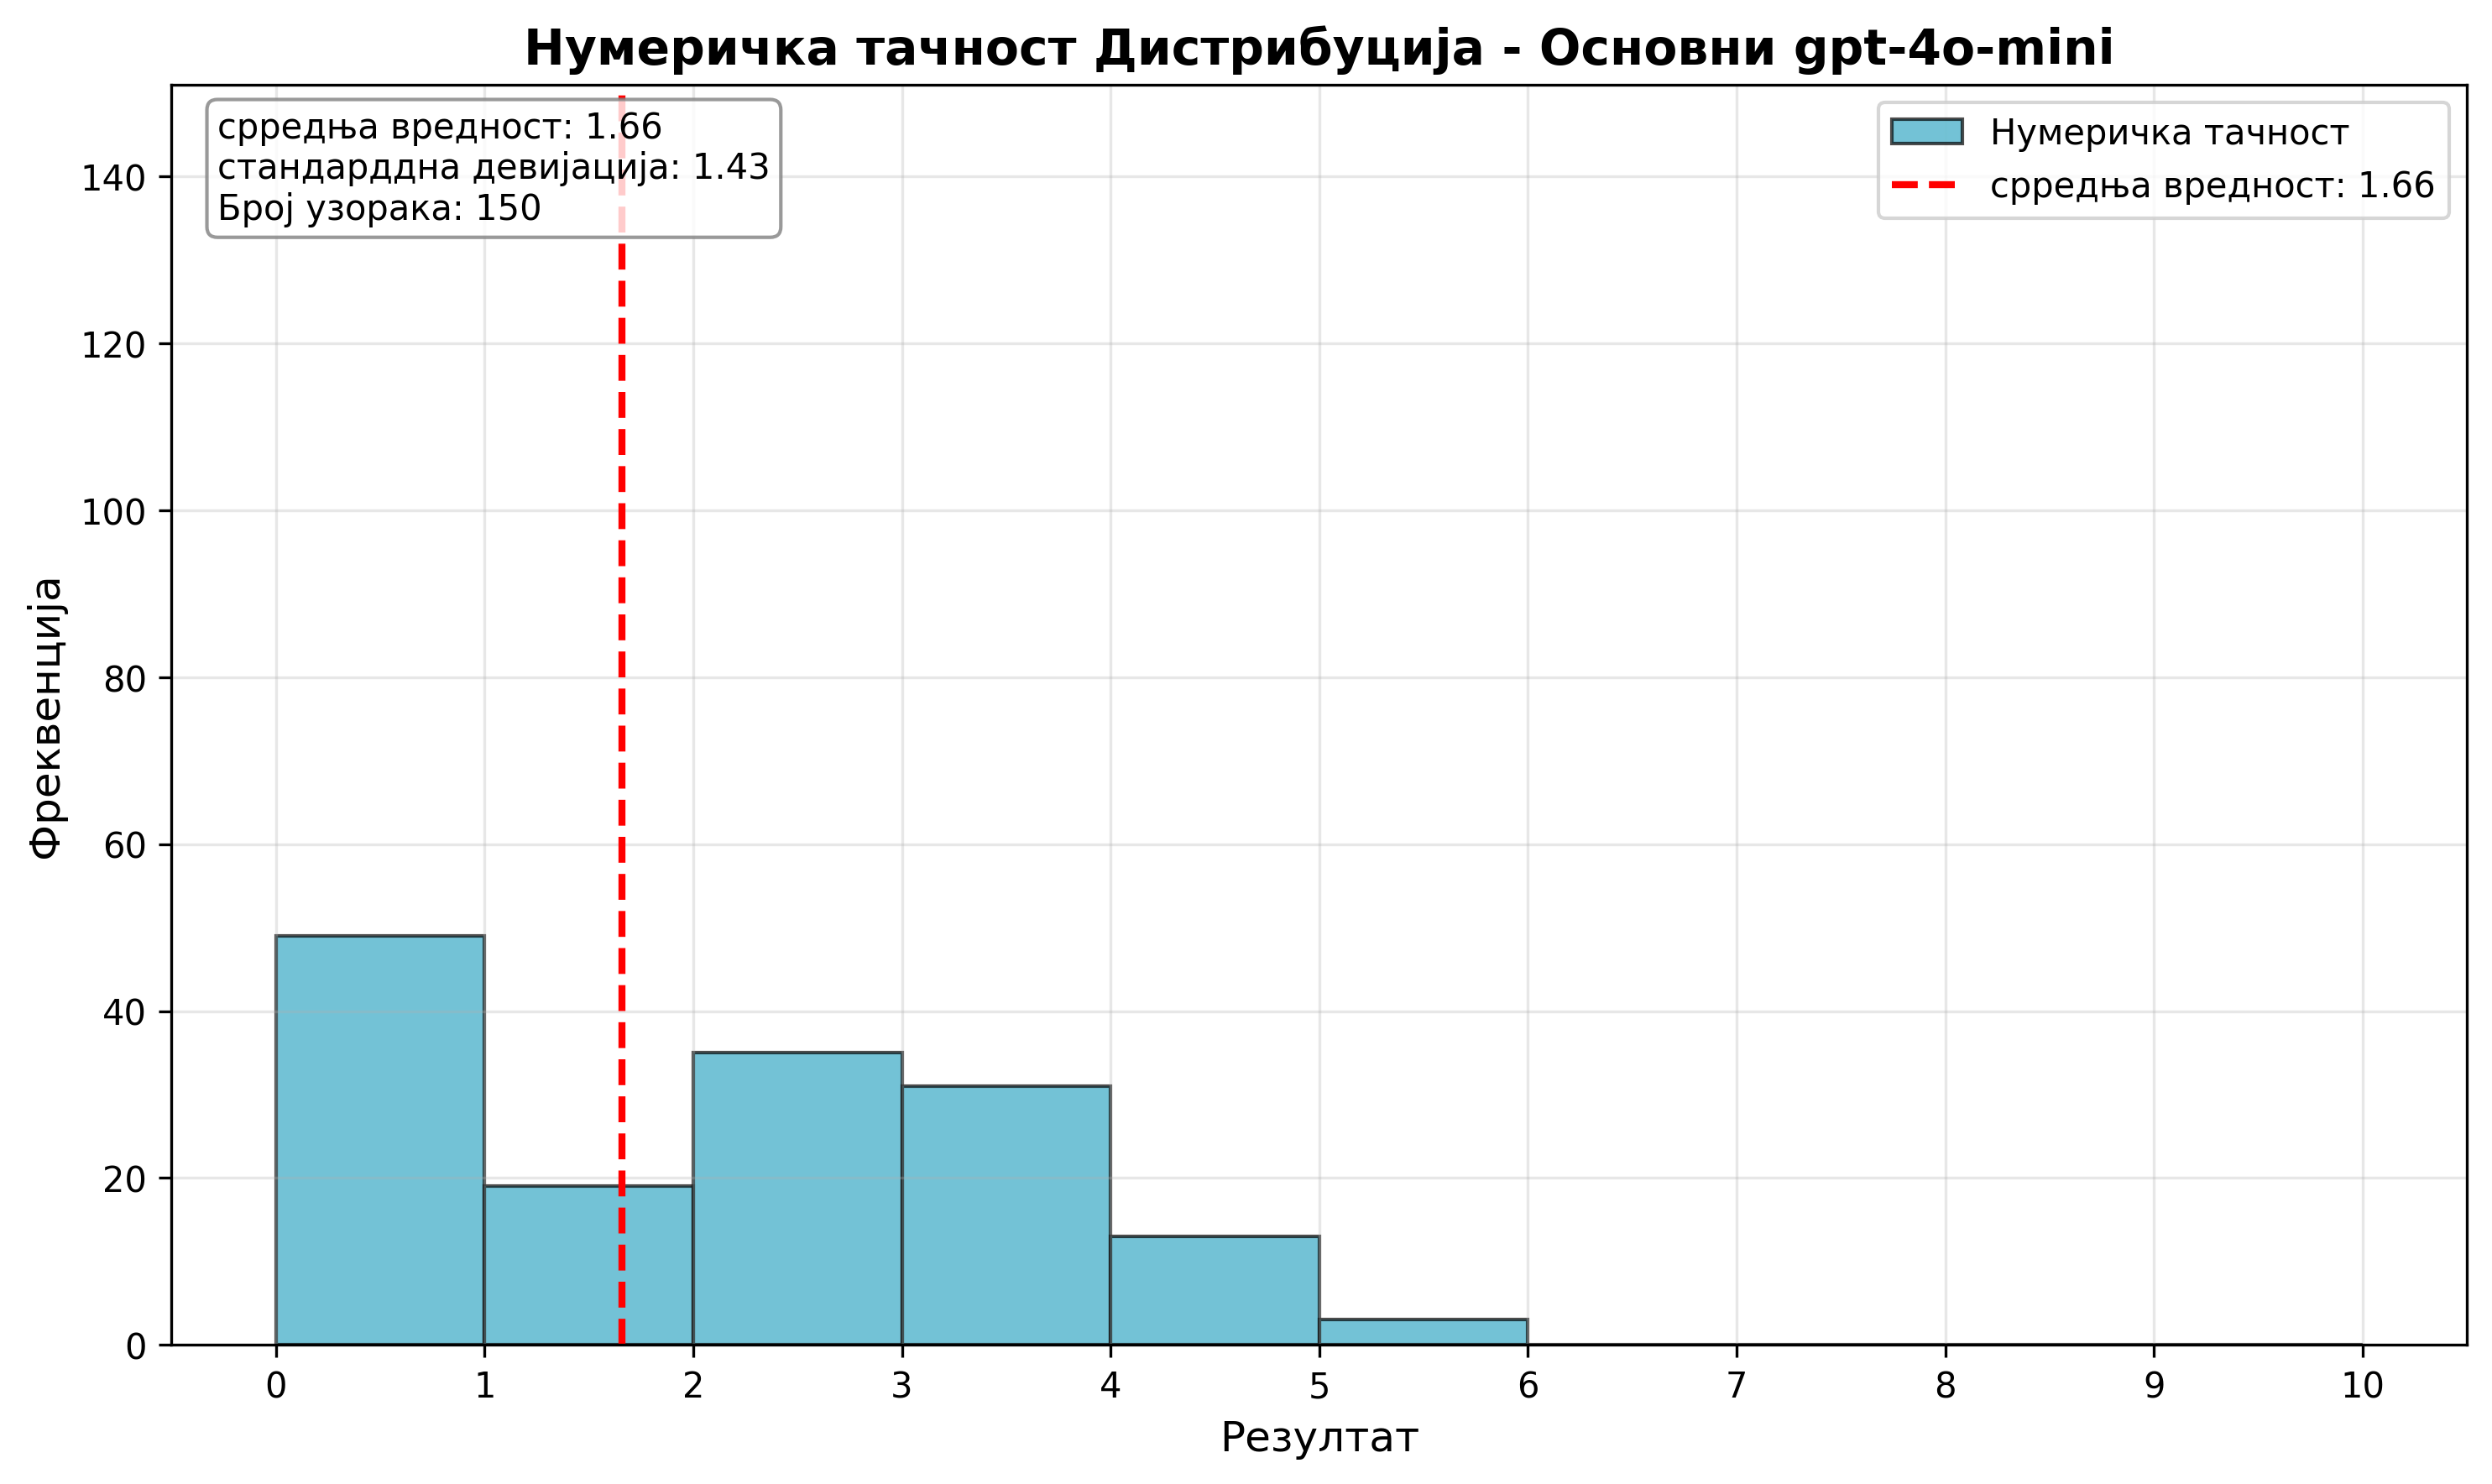
\includegraphics[width=0.8\textwidth]{images/osnovni/criteria_analysis_numerical_accuracy_histogram.png}
    
    \vspace{0.5cm}
    
    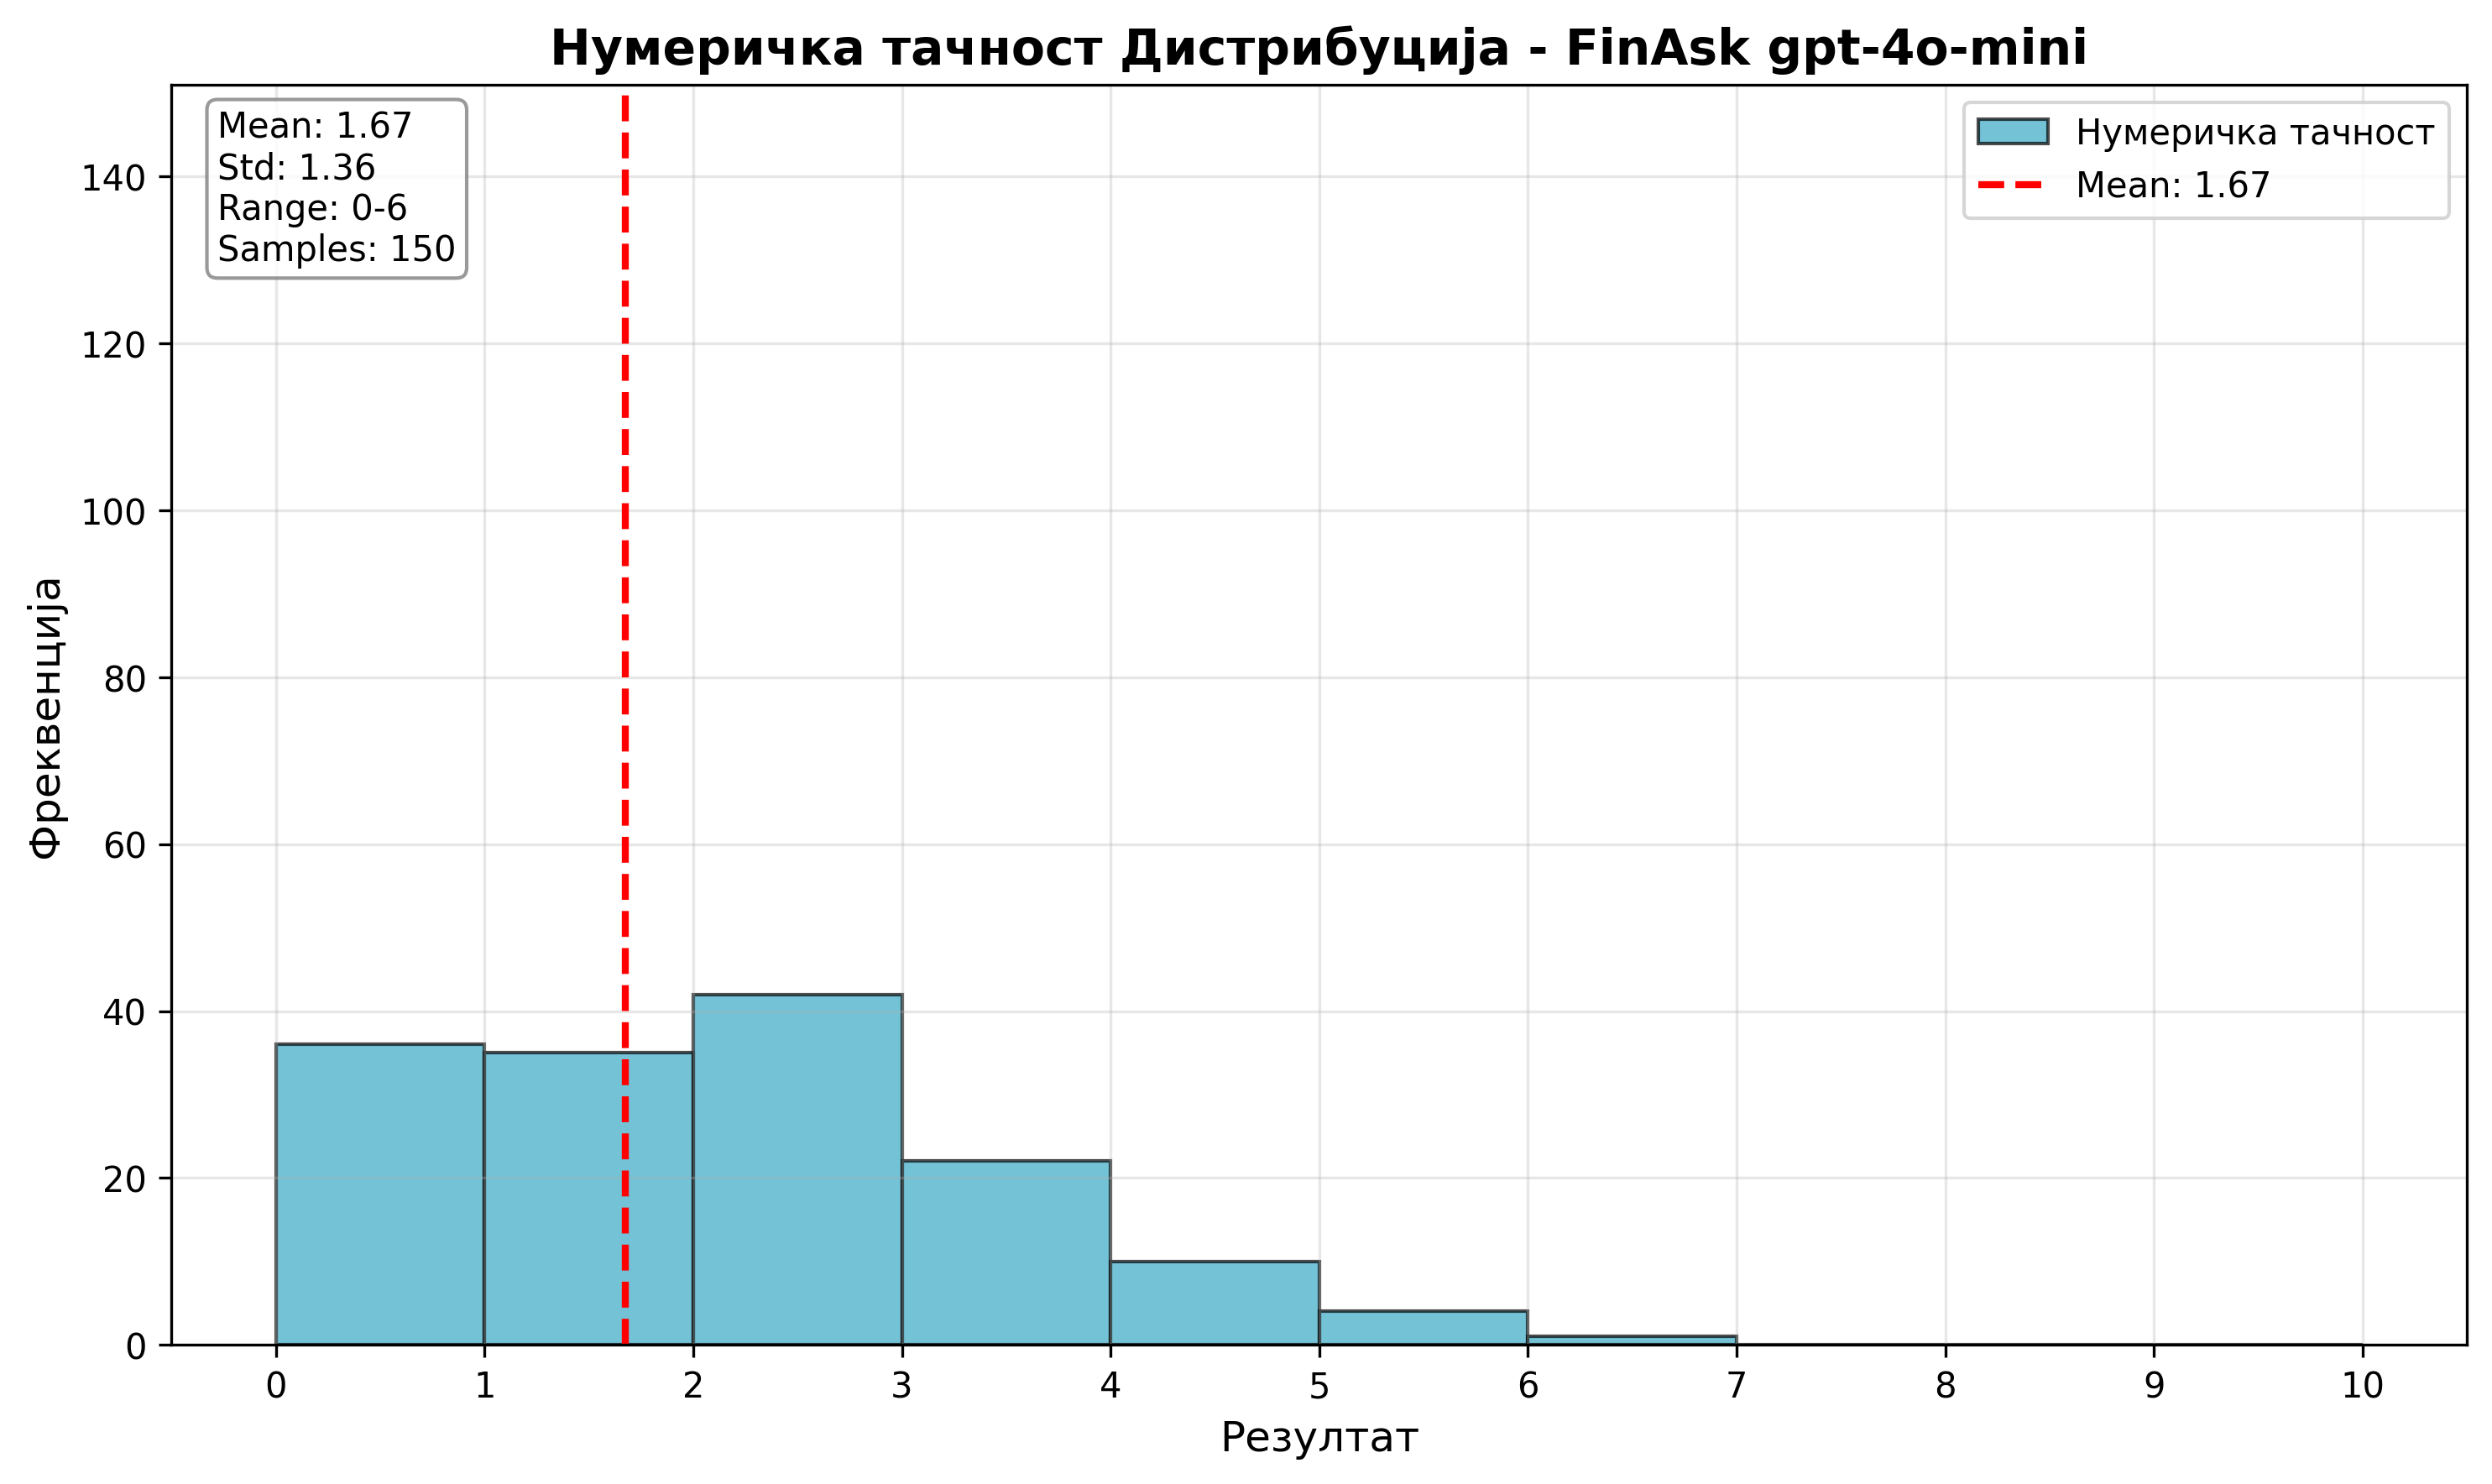
\includegraphics[width=0.8\textwidth]{images/FinAsk/criteria_analysis_numerical_accuracy_histogram.png}
    \caption{Хистограм анализе критеријума нумеричке тачности - горе: основни модел, доле: FinAsk модел}
    \label{fig:comparison_numerical}
\end{figure}